\chapter{Particle Identification}
% -----------------------------------------
%    chapter motivation and purpose 
% -----------------------------------------

\section{Introduction}
Particle identification (PID) is the process of classifying tracks as known particles.  After reconstruction and matching of detector responses to each track, the reconstruction package \texttt{recsis} assigns a preliminary particle identification based on loose selection criteria.  In this analysis, tracks are classified based on a more stringent criteria.  This chapter discusses the methodology used to classify particles.  

\section{Electron Identification}
Electrons in CLAS are abundant, and the detection of an electron is a basic necessity for every event that will be analyzed.  The most naive approach to performing electron identification would be to call all negatively charged tracks electrons.  Doing this would provide an extremely efficient identification of electrons (none of them are missed), however the purity of the sample (the fraction of tracks identified as electrons that are actually electrons) would be low due to the vast quantity of negatively charged pions that are produced in during the experiment.  Additionally, doing this would completely eliminate the possibility of identifying negatively charged pions or kaons, as all negative tracks would be called electrons.  In practice then, the identification of electrons is concerned with removal of negative pions and kaons from the sample of negative tracks.  This is accomplished by applying a series of cuts on measured variables that distinguish between electrons and pions (pions are the dominant background).

\subsection{Electron ID Cuts}
The cuts used to select electrons are enumerated below.

\begin{itemize}
  \item{Negative charge}
  \item{Drift chamber region 1 fiducial}
  \item{Drift chamber region 3 fiducial}
  \item{Electromagnetic Calorimeter fiducial (UVW)}
  \item{EC minimum energy deposition}
  \item{Sampling Fraction (momentum dependent)}
  \item{z-vertex position}
  \item{Cherenkov counter $\theta_{cc}$ matching to PMT number}
  \item{Cherenkov counter $\phi_{rel}$ matching to PMT (left/right)}
  \item{Cherenkov counter Fiducial Cuts}
\end{itemize}

Each cut is now be described in more detail.

\subsubsection*{Negativity Cut}
Each track is assigned a charge based on the curvature of its trajectory through the magnetic field of the torus.  This is done during the track reconstruction phase.  Tracks are eliminated as electron candidates if they are not negatively charged.

\subsubsection*{Drift chamber fiducial}
The fiducial region or volume is a term used to refer to the region of a sensitive detector which is unimpeded in its acceptance of physics events.  In practice, shadows from other detectors, poorly understood edge effects, or geometric obstacles may impede the flight of particles from the target, and render regions of sensitive detectors unreliable (to use the vocabulary presented above, these events fall outside of the fiducial region of the detector).  \\

Negative tracks which pass geometrically close to the edges of the drift chamber are, from a tracking perspective, more difficult to understand.  Additionally, tracks which fall outside of the fiducial region of the drift chambers are likely to fall outside of the fiducial region of the downstream detectors as well.  For these reasons, it is common to remove tracks which are geometrically close to the boundaries of the drift chambers in region 1 as well as region 3 coordinate systems.\\

To implement this cut the $(x,y)$ coordinates of the drift chambers are rotated into one sector.  Then boundaries $y_{left}, y_{right}$ are defined as linear functions of $x$. The boundary lines are parametrized by an offset $h$ and an angle of the boundary line with respect to the center of the sector at $x = 0$.  The slope of these lines is $\pm \cot(\theta)$.  

\begin{eqnarray}
  y_{right} = h + \cot(\theta) x \\
  y_{left} = h - \cot(\theta) x
\end{eqnarray}

Tracks passing this criterion are those which have $y > y_{left}(x)$ and $y > y_{right}(x)$.  

\begin{table}
  \centering
  \begin{tabular}{c|c|c}
    Region & Height $h$ (cm) & Angle $\theta$ (degrees)\\
    \hline 
    1 & 22 & 60 \\
    3 & 80 & 49
  \end{tabular}
  \caption{Cut parameters used for the DC fiducial cut.}
\end{table}

\easyFigure{image/plots/electron-id/summary-dc-region1.pdf}{Tracks shown in color remain after the application of drift chamber region 1 fiducial cuts to all cuts, shown here as black points.}
\easyFigure{image/plots/electron-id/summary-dc-region3.pdf}{The selection criteria shown in red is applied to drift chamber region 3.}

\subsubsection*{Electromagnetic Calorimeter fiducial (UVW)}
As particles traverse the electromagnetic calorimeter they develop electromagnetic showers.  If the track passes close to the edges of the detector, there is a chance that the shower will not be fully contained within the calorimeter volume (it spills out the edges).  For this reason, it is standard to remove the hits which fall within the outer 10 centimeters of each layer of the EC (10 centimieters is the width of a scintillator bar).  This cut is applied in the U, V, W coordinate system.  

\begin{table}
  \centering
  \begin{tabular}{c|c|c}
    EC Coordinate & Min (cm) & Max (cm) \\
    \hline 
    U & 70 & 400 \\
    V & - & 362 \\
    W & - & 395
  \end{tbular}
  \caption{Cut parameters used for the EC fiducial cut.}
\end{table}

\easyFigure{image/plots/electron-id/ec-fid.png}{All negative tracks are shown here in black.  In color, the tracks which pass the EC fiducial cut are shown.}

\subsubsection*{EC minimum energy deposition}
One way to differentiate between these electrons and pions is to exploit the difference in energy deposition between the two in the electromagnetic calorimeter.  Electron typically develop a much larger and more energetic shower than $\pi$ mesons, which minimally ionize the calorimeter material.  The result is that the total energy deposition is typically larger for electrons than $\pi$ mesons.  In this analysis we require that at least 60 MeV was deposited in the inner calorimeter for electron candidates \ref{fig:ec-edep}.  

\begin{figure}
	\centering
	\label{fig:ec-edep}
	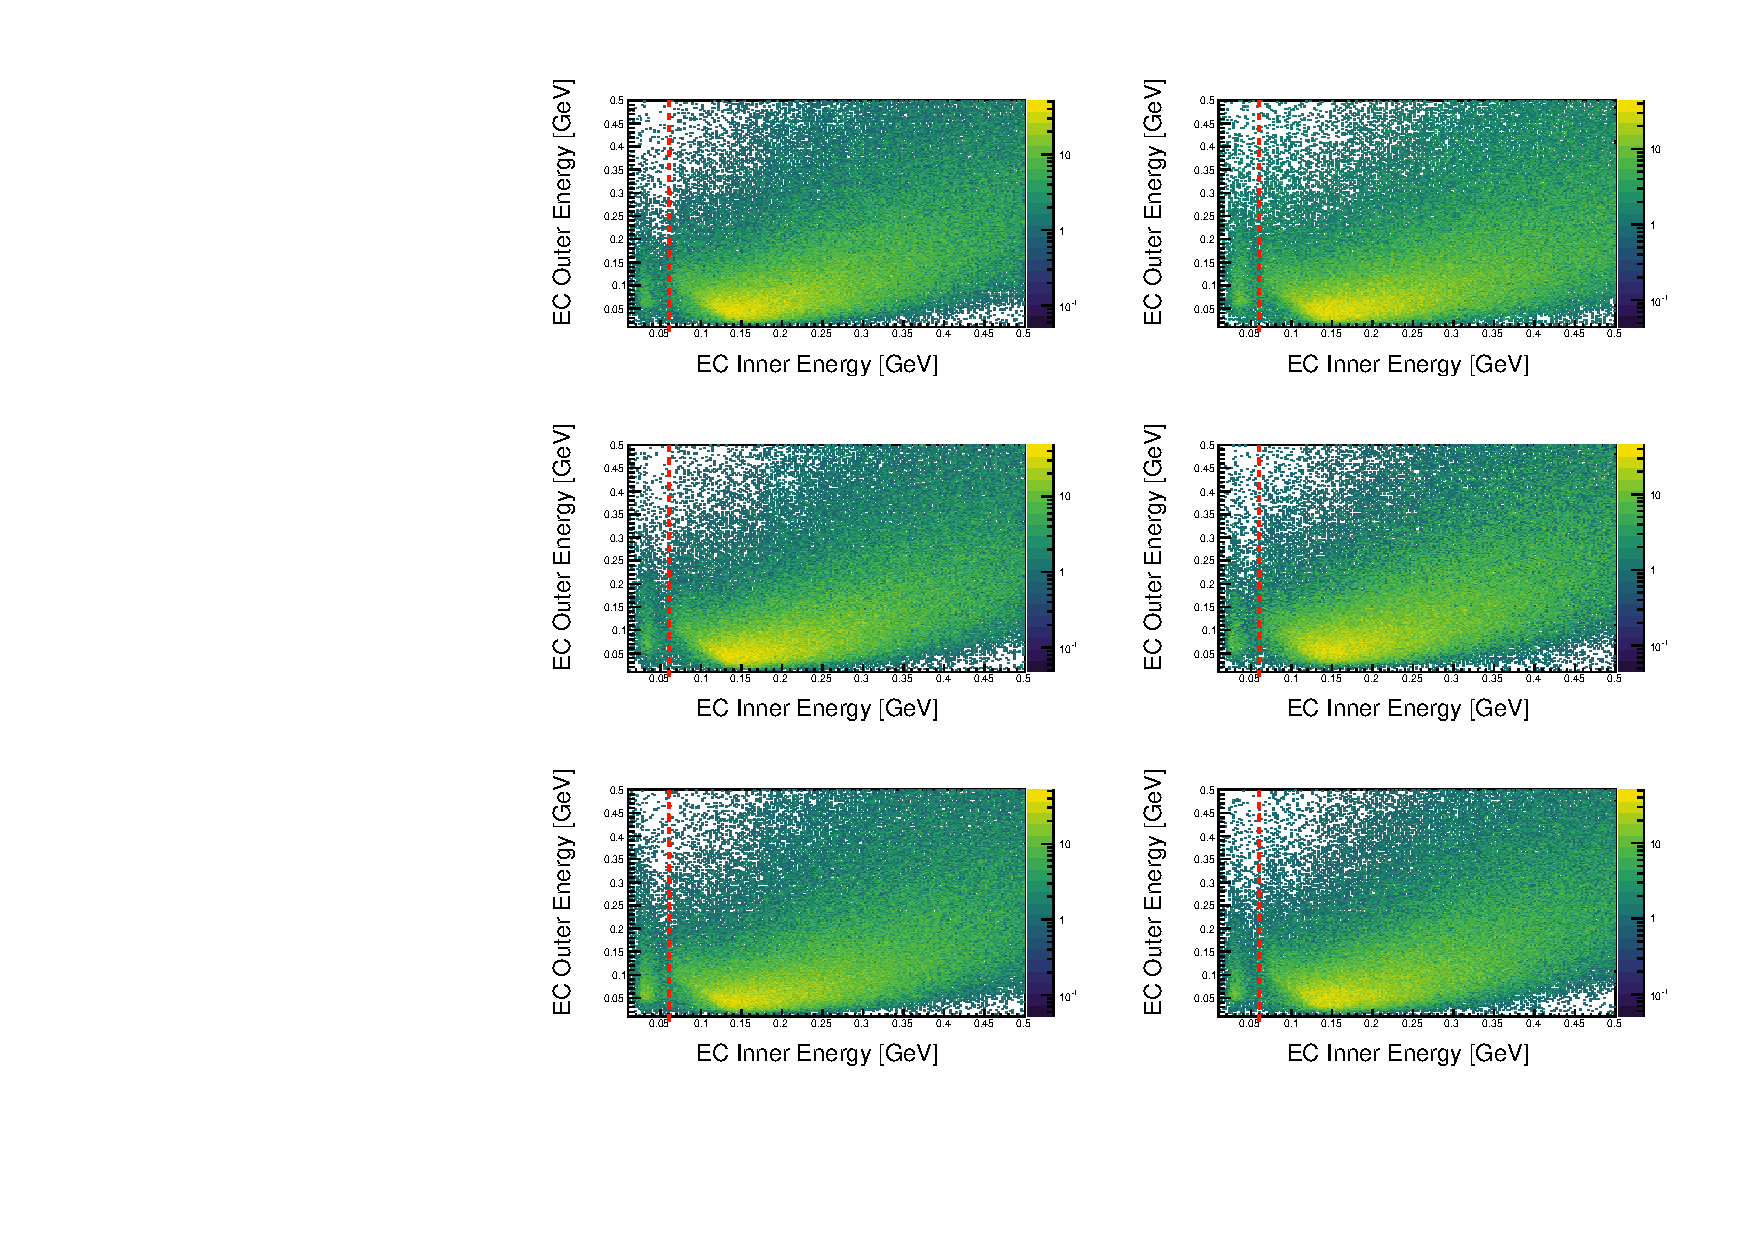
\includegraphics[width=\textwidth]{image/plots/summary-ec-edep.pdf}
	\caption{Each panel shown above contains events from one sector, increasing from 1-6 from top left to bottom right.  The value selected of 60 MeV is applied to all sectors and separates the negatively charged pions (left) from the electrons (right).}
\end{figure}

\subsubsection*{Sampling Fraction (momentum dependent)}
The electromagnetic calorimeter is designed such that electrons will deposit $E_{dep}/p \approx 0.3$ approximately one-third of their energy, regardless of their momentum.  In contrast to this, the ratio $E_{dep}/p$ for $\pi$ mesons decreases rapidly with momentum.  To develop a momentum dependent cut for this distribution, all negative candidates are first filled into a two-dimensional histogram of $E_{dep}/p$ vs. $p$.  The histogram is then binned more coarsely in momentum, and projected into a series of 40 momentum slices.  Each of these slices is fit with a Gaussian to extract the position $\mu_i$ and width $\sigma_i$ of the electron peak.  Finally, a functional form for the mean and standard deviation of the distributions is chosen to be a third order polynomial in momentum.

\begin{eqnarray}
  \mu (p) = \mu_0 + \mu_1 p + \mu_2 p^2 + \mu_3 p^3 \\
  \sigma (p) = \sigma_0 + \sigma_1 p + \sigma_2 p^2 + \sigma_3 p^3 
\end{eqnarray}    

Boundaries are constructed from this information by adding (subtracting) $n_{\sigma}$ from the mean.  In the nominal case, we use $n_{\sigma} = 2.5$.

\begin{eqnarray}
  f_{max} (p) = \mu (p) + n_{\sigma} \sigma (p) = (\mu_0 + n_{\sigma} \sigma_0) + (\mu_1 + n_{\sigma} \sigma_1)p + (\mu_2 + n_{\sigma} \sigma_2)p^2 + (\mu_3 + n_{\sigma} \sigma_3)p^3 \\
  f_{min} (p) = \mu (p) - n_{\sigma} \sigma (p) = (\mu_0 - n_{\sigma} \sigma_0) + (\mu_1 - n_{\sigma} \sigma_1)p + (\mu_2 - n_{\sigma} \sigma_2)p^2 + (\mu_3 - n_{\sigma} \sigma_3)p^3
\end{eqnarray}

Due to slight differences between the 6 sectors of the CLAS detector, this cut is calibrated and applied for each sector individually.  Results are shown in table \ref{table-sampling-fraction}.

\easyFigure{image/plots/electron-id/summary-sampling-fraction.pdf}{The sampling fraction selection boundary is shown here for the nominal value of $N_{sigma} = 4$.}

% ---------------------------------
%  table of cut values for this 
% ---------------------------------

\begin{table}[h]
  \centering 

  \begin{tabular}{c | c | c | c | c | c | c}
    Parameter & Sector 1 & Sector 2 & Sector 3 & Sector 4 & Sector 5 & Sector 6                           \\
    \hline
    $\mu_3$     & -8.68739e-05 & 0.000459313  &  9.94077e-05 & -0.000244192 & -7.65218e-05 & -0.000392285  \\
    $\mu_2$     & -0.000338957 & -0.00621419  & -0.00267522  & -0.00103803  & -0.00222768  & -0.00105459   \\
    $\mu_1$     &  0.0191726   &  0.0393975   &  0.02881     &  0.0250629   &  0.0233171   &  0.0265662    \\
    $\mu_0$     &  0.2731      &  0.296993    &  0.285039    &  0.276795    &  0.266246    &  0.25919      \\
    $\sigma_3$  & -0.000737136 &  0.000189105 & -0.000472738 & -0.000553545 & -0.000646591 & -0.000633567  \\
    $\sigma_2$  &  0.00676769  & -0.000244009 &  0.00493599  &  0.00434321  &  0.00717978  &  0.00626044   \\
    $\sigma_1$  & -0.0219814   & -0.00681518  & -0.0180929   & -0.0140827   & -0.0246181   & -0.022029     \\
    $\sigma_0$  &  0.0474188   &  0.0475098   &  0.0461743   &  0.0492728   &  0.0546257   &  0.0517508    
  \end{tabular}
  \caption{$\mu$ and $\sigma$ values used to construct the momentum dependent sampling fraction cut.}
  \label{table-sampling-fraction}
\end{table}

\subsubsection*{z-vertex position}
Electrons can be produced as part of $e^+ e^-$ pairs, or by other processes.  For this analysis, these are not of interest.  For the purposes of this analysis it is then natural to accept only electron candidates which have a z-vertex $v_z \in [-27.7302, -22.6864]$ within the expected target region.  This cut is applied after the vertex position has been corrected (which is discussed in the basic analysis section).

\easyFigure{image/plots/electron-id/summary-z-vertex.pdf}{The track vertex cut is shown above.  All negative tracks are shown in white, while the tracks passing all other criteria are shown in black hatch.  The cut bounday is displayed as red lines.  For E1-F the target center was located at -25 cm.}

\subsubsection*{Cherenkov counter fiducial cuts}
The value of the polar angle $\theta_{cc}$ and the azimuthal angle $\phi_{rel}$ with respect to the center of the sector is used for each event to define a fiducial cut at the Cherenkov counter.  In this study, the functional form below is used for the boundary function.

\begin{equation}
	\theta_{cc} > 46 - 35 \sqrt{1 - \phi_{rel}^2  / 350}
\end{equation} 

The parameters were chosen empirically based on a study of the distributions with and without other electron identification cuts applied.

\subsubsection*{Cherenkov counter $\theta_{cc}$ and $\phi_{rel}$ matching to PMT}
The angular arrangement of photo-multiplier tubes (PMTs) in the Cherenkov counter allows for additional consistency conditions to be applied.  Each half-sector of the CC contains 18 PMTs increasing in polar angle away from the beamline, these divisions are known as segments.  The polar angle measured at the Cherenkov counter $\theta{cc}$ is then correlated to the segment in which the track was detected.  Additionally, PMTs that are placed on the left and right of the detector can be used to check consistency with the azimuthal angle the track forms with the central line of the detector (ie $\phi_{rel} > 0$ means the track was in the right half of the sector, $\phi_{rel} < 0$ means the track was in the left half of the sector).  An integer is used to describe the PMT associated with the track.  The left PMT is assigned value -1, the right 1, and a signal in both PMTs is assigned 0.  If both PMTs have a signal, the track is allowed to pass.  If the left PMT was the one that had a signal, only events with $\phi_{rel} < 0$ passes.  Similarly if the right PMT fired (code = 1), only events with $\phi_{rel} > 0$ are allowed to pass. 

\easyFigure{image/diagrams/relative-phi.pdf}{The angle $\phi_{rel}$ is the azimuthal angle between the central line of the detector and the track.}
\easyFigure{image/plots/electron-id/summary-cc-theta.pdf}{Correlation between $\theta_{CC}$ and the CC segment is shown above, with our selection boundaries overlaid in red.}

% ------------------------------------
%      Inclusive Cross Section
% ------------------------------------
\section{Inclusive Electron Cross Section}
A brief discussion is provided here regarding our extraction of the inclusive electron scattering cross section in the resonance region.  The inclusion of this study here is intended to add credibility to our electron identification and good run list.  Inclusive electron scattering is the process $e p \rightarrow e X$, where only the final state electron is detected and the rest of the event is not (anything apart from the electron that is detected is not analyzed).  As a function of $W$ (the invariant mass of the final state ($\gamma^* + p$) system) the region below 2 GeV contains resonances and is often referred to as the resonance region.  Resonance structures are difficult to detect higher than about 2 GeV, and this region is typically called the \textit{deeply inelastic} region.  While the deeply inelastic region is used extensively for measurements in nuclear/particle physics, the goal of luminosity and electron identification verification is more easily achieved in the resonance region.  This fact is due principally to the excess of Bethe-Heitler events which collect in the $2 < W < 3$ region for $E_{beam} = 5.498$ (such events are difficult to remove when detecting only the final state electron).  The cross section is measured by counting events in each kinematic bin, and normalizing by the integrated luminosity over files analyzed.  Additionally, acceptance and radiative corrections are applied bin-by-bin as shown in \ref{eqn:cross_section_measured}.

\begin{equation}
	\label{eqn:cross_section_measured}
	\frac{d^2 \sigma}{dW \; dQ^2} = \frac{1}{\Delta W \; \Delta Q^2} \frac{N_{i}}{\mathcal{L} \; A_i \; R_i}
\end{equation}

Here $A_i$ and $R_i$ refer to the acceptance and radiative corrections for the bin $i$, and $\mathcal{L}$ is the integrated luminosity.  

\subsubsection*{Event Selection and Binning}
A simple choice of 10 bins in $Q^2$ and 40 bins in $W$ is used.  This choice is mainly driven by the desire to keep bin migration effects small.  Events are generated and reconstructed in some bins $R^{(j)}$ and $G^{(i)}$ respectively.  Due to finite detector resolution, it is not always the case that $i = j$.  This effect is known as bin migration, and negatively impacts the acceptance calculation.\\
The only kinematic restriction that is imposed is applied to the \textit{inelasticity} $y = 1-E'/E < 0.7$.  This restriction is applied because events with large-$y$ have a significantly higher probability to be Bethe-Heitler events.  This cut is equivalent to enforcing a minimum energy for the scattered electron.

\begin{equation}
        E_{min} = E_{beam}(1-y_{max}) \approx 1.6 \; GeV
\end{equation}

\begin{table}
  \centering
  \begin{tabular}{c|c|c|c|c}
    Variable & N & Min. & Max & Width \\
    \hline
    $W$   & 40 & 1.1 & 2.1 & 0.25 \\
    $Q^2$ & 10 & 1.7 & 4.2 & 0.25
  \end{tabular}
  \caption{Summary of $W$ and $Q^2$ binning used for the inclusive cross section.}
\end{table}

\subsubsection*{Results}
All sectors individually were analyzed and our results are consistent with the model parametrization by Cynthia Keppel \ref{fig:inclusive_xs}.  In most of the kinematics that we studied, our extracted cross section is within 5 \% of the model prediction.  The most notable difficulty that appeared was the residual elastic tail at lower $W$ values that caused some kinematic bins to be slightly off.  There also exist bin migration effects on the resonance peaks, but these are small.

\begin{sidewaysfigure}
	\begin{center}
		\label{fig:inclusive_xs}
		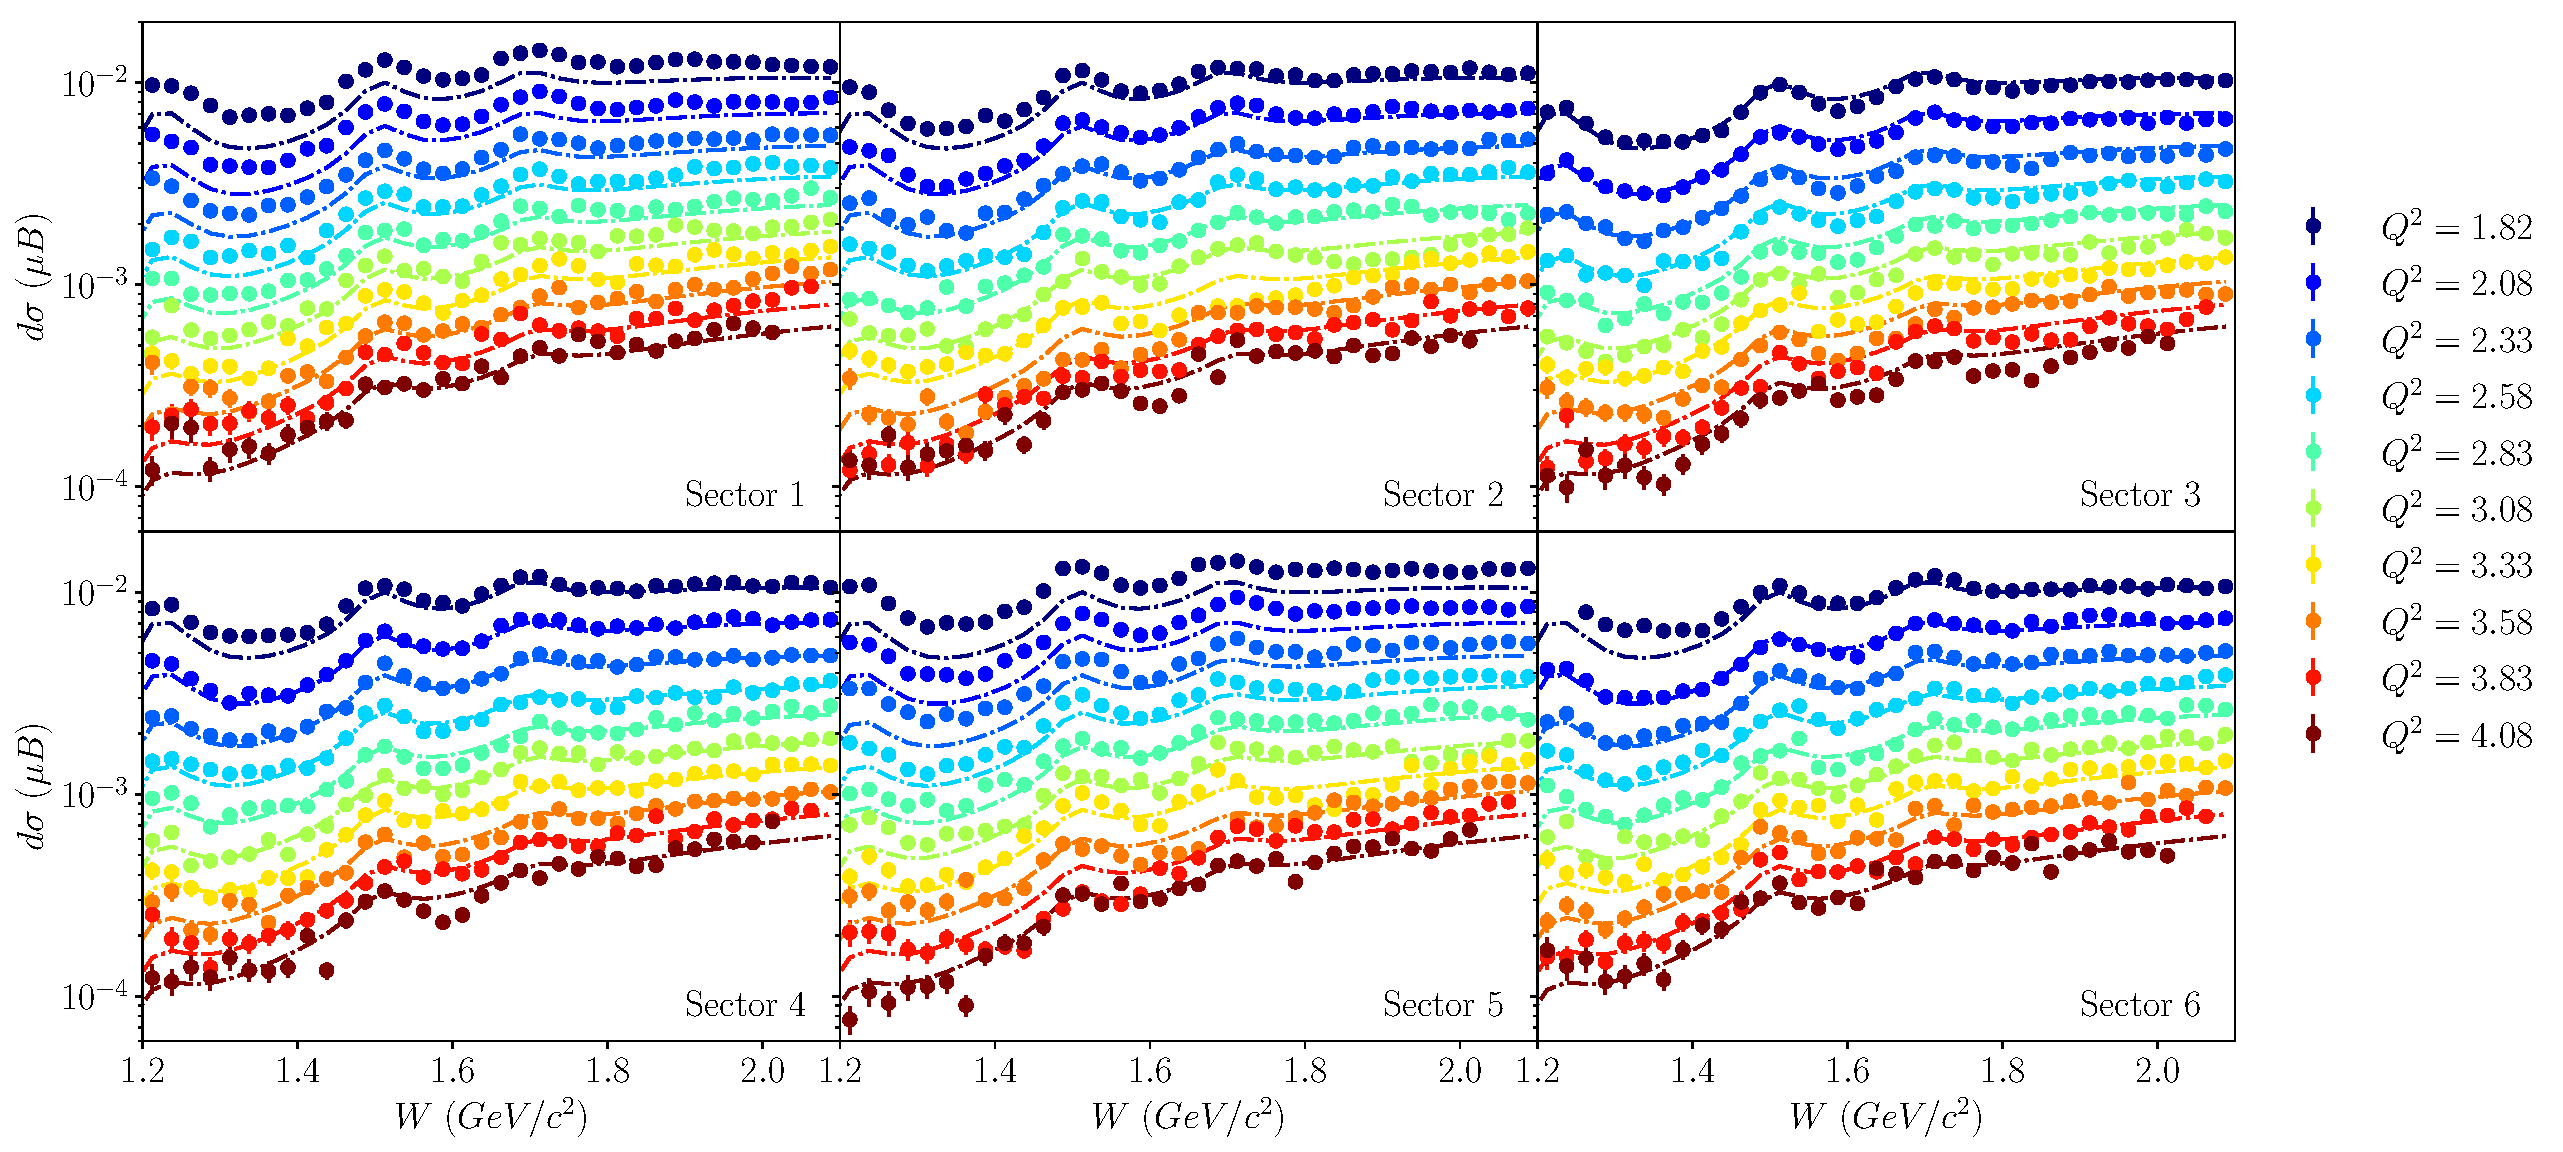
\includegraphics[width=\textwidth]{image/plots/inclusive/inclusive_xs.pdf}	
		\caption{Inclusive cross section results compared with model predictions.  Each panel shows the result for all 10 $Q^2$ bins and one sector.}
	\end{center}
\end{sidewaysfigure}

% ------------------------------------
%     Hadron ID
% ------------------------------------
\section{Hadron Identification}
Hadron identification in CLAS is done by correlating particle momentum from the drift chambers with timing information supplied by the time of flight detector.  In this analysis some quality assurance cuts are applied preliminarily, but they do not discriminate between different species of particle.  The likelihood methodology described in this section is based on the discussion provided by the BES collaboration in \cite{misc-ping:2009}.  

\subsection{Hadron ID Cuts}
The cuts used for hadron classification are enumerated below.

\begin{itemize}
  \item{Drift chamber fiducial}
  \item{Hadron-electron vertex difference}
  \item{Likelihood maximization of $\beta(p,h)$}
\end{itemize}


\subsubsection*{Drift chamber fiducial}
Drift chamber fiducial cuts are applied (only region 1) using the same procedure as described for electrons.  The parameters used for positive tracks are $h = 10$, $\theta = 60$.

\begin{figure}
  \label{fig:fid}
  \begin{center}
    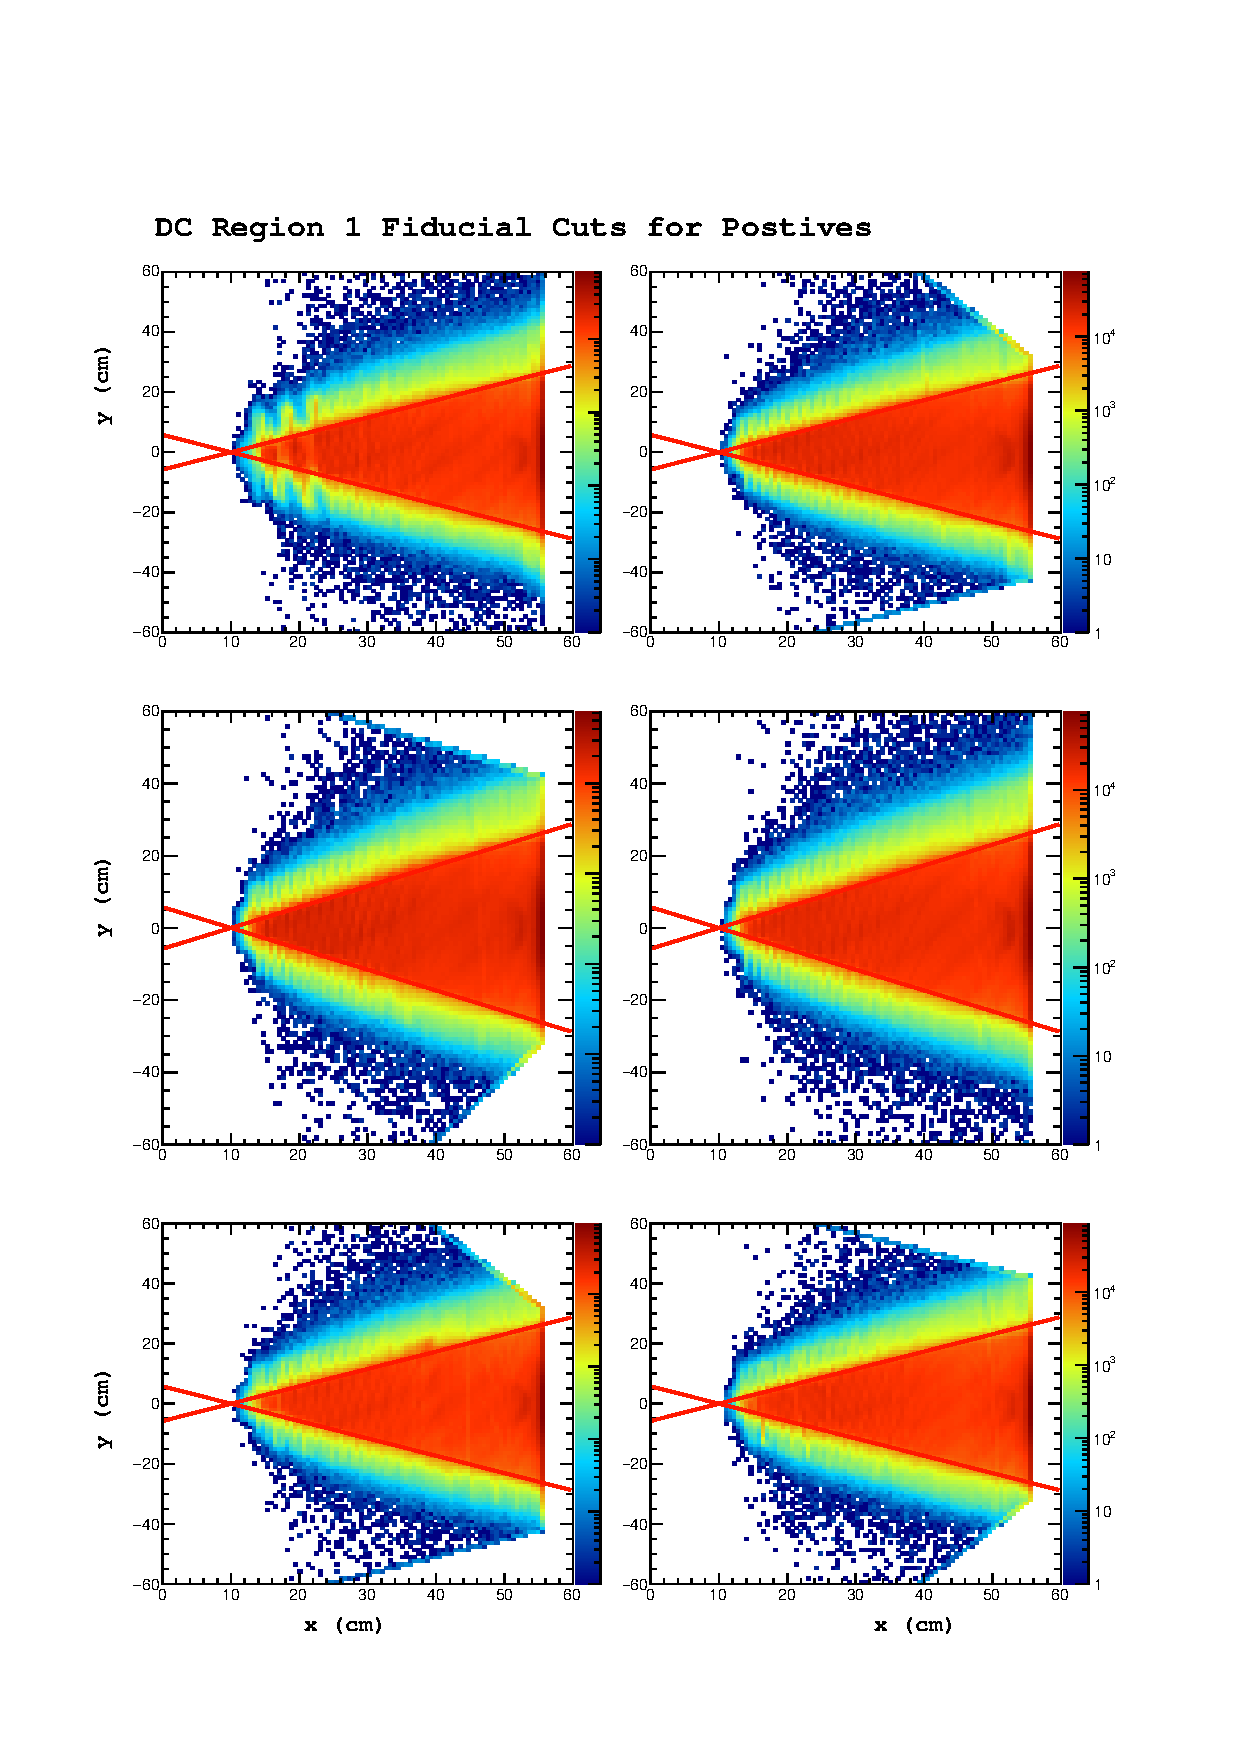
\includegraphics[width=10cm]{image/plots/hadron-id/fid.pdf}
    \caption{Positive track hits on the region 1 drift chamber, events falling between the red lines are kept for analysis.}
  \end{center}
\end{figure}

\subsubsection*{Hadron-electron vertex difference}
The distance between the electron vertex and the hadron candidate track vertex is computed ($\delta v_{z} = v_{z}^{e} - v_{z}^{+}$).  This distance is constrained to be within the length of the target (5 cm) see figure \ref{fig:dvz}.  For events where the electron-kaon vertex difference is larger than the target size, we cannot assert that the kaon came from the electron-proton collision.  Although the number of events excluded by this cut is not large, those events are considered to be outliers.  

\begin{figure}
  \label{fig:dvz}
  \begin{center}
    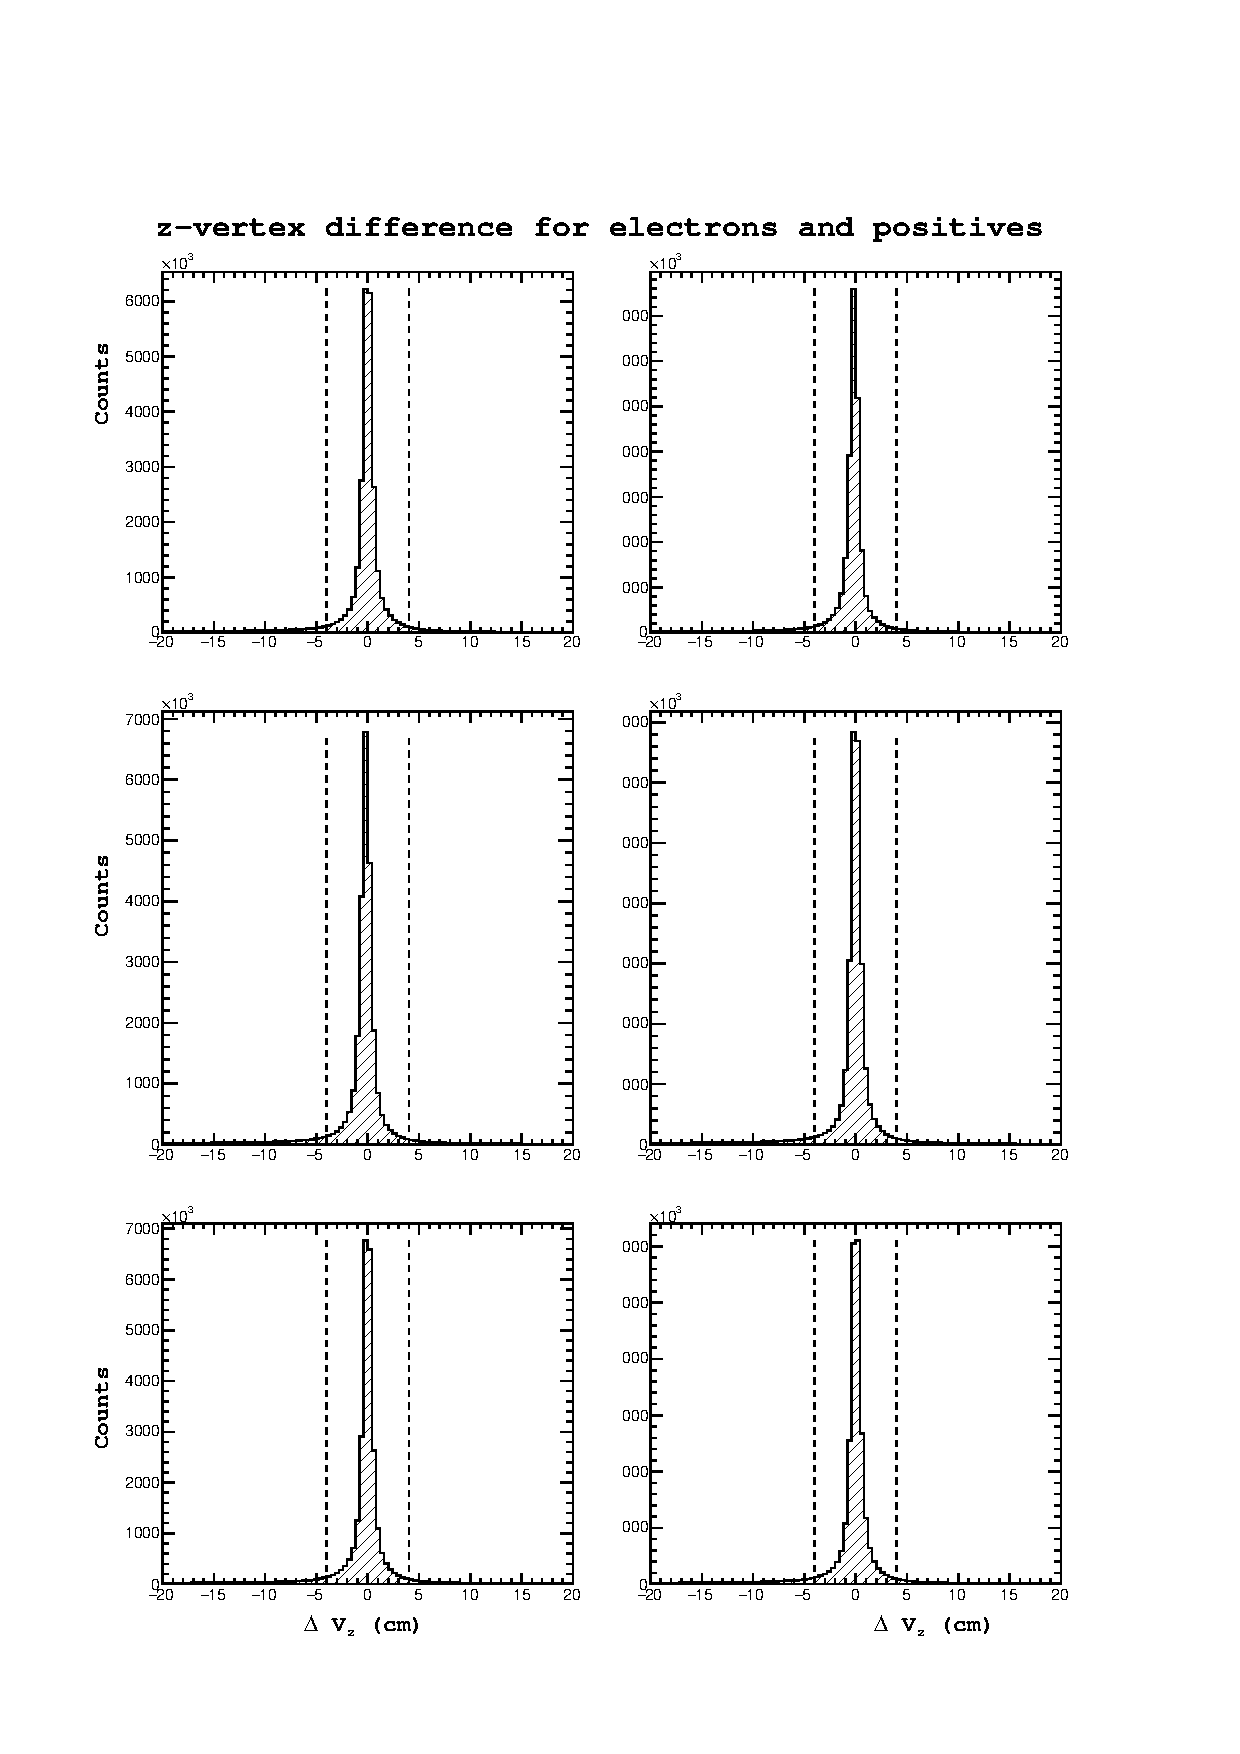
\includegraphics[width=10cm]{image/plots/hadron-id/dvz.pdf}
    \caption{The difference between the z-vertex position between detected electrons and positive tracks.}
  \end{center}
\end{figure}



% These really don't add anything to the discussion 
%
%\begin{figure}
%	\label{fig:beta_p_dvz}
%  \begin{center}
%    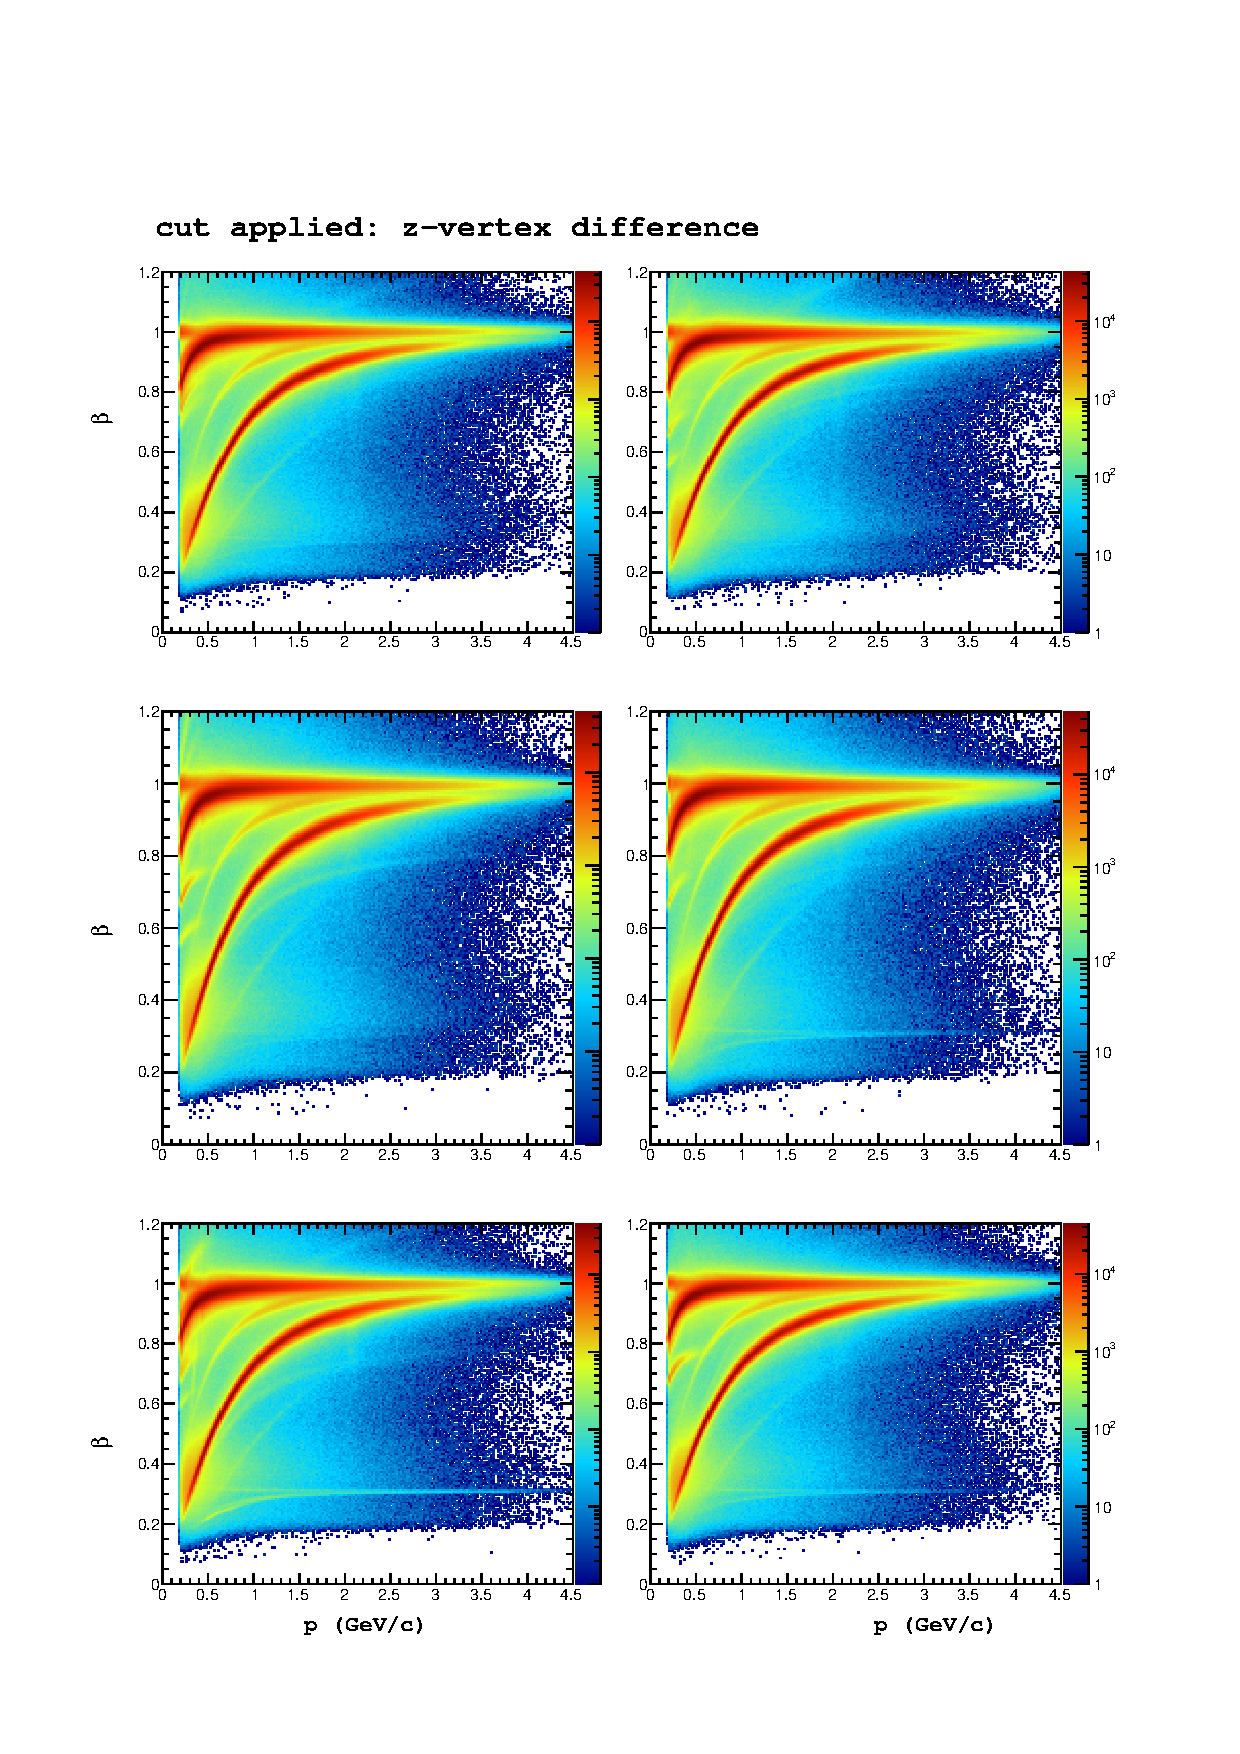
\includegraphics[width=10cm]{image/plots/hadron-id/p_beta_dvz.pdf}
%    \caption{Shown above: Something.}
%\end{center}
%\end{figure}

%\begin{figure}
%  \begin{center}
%    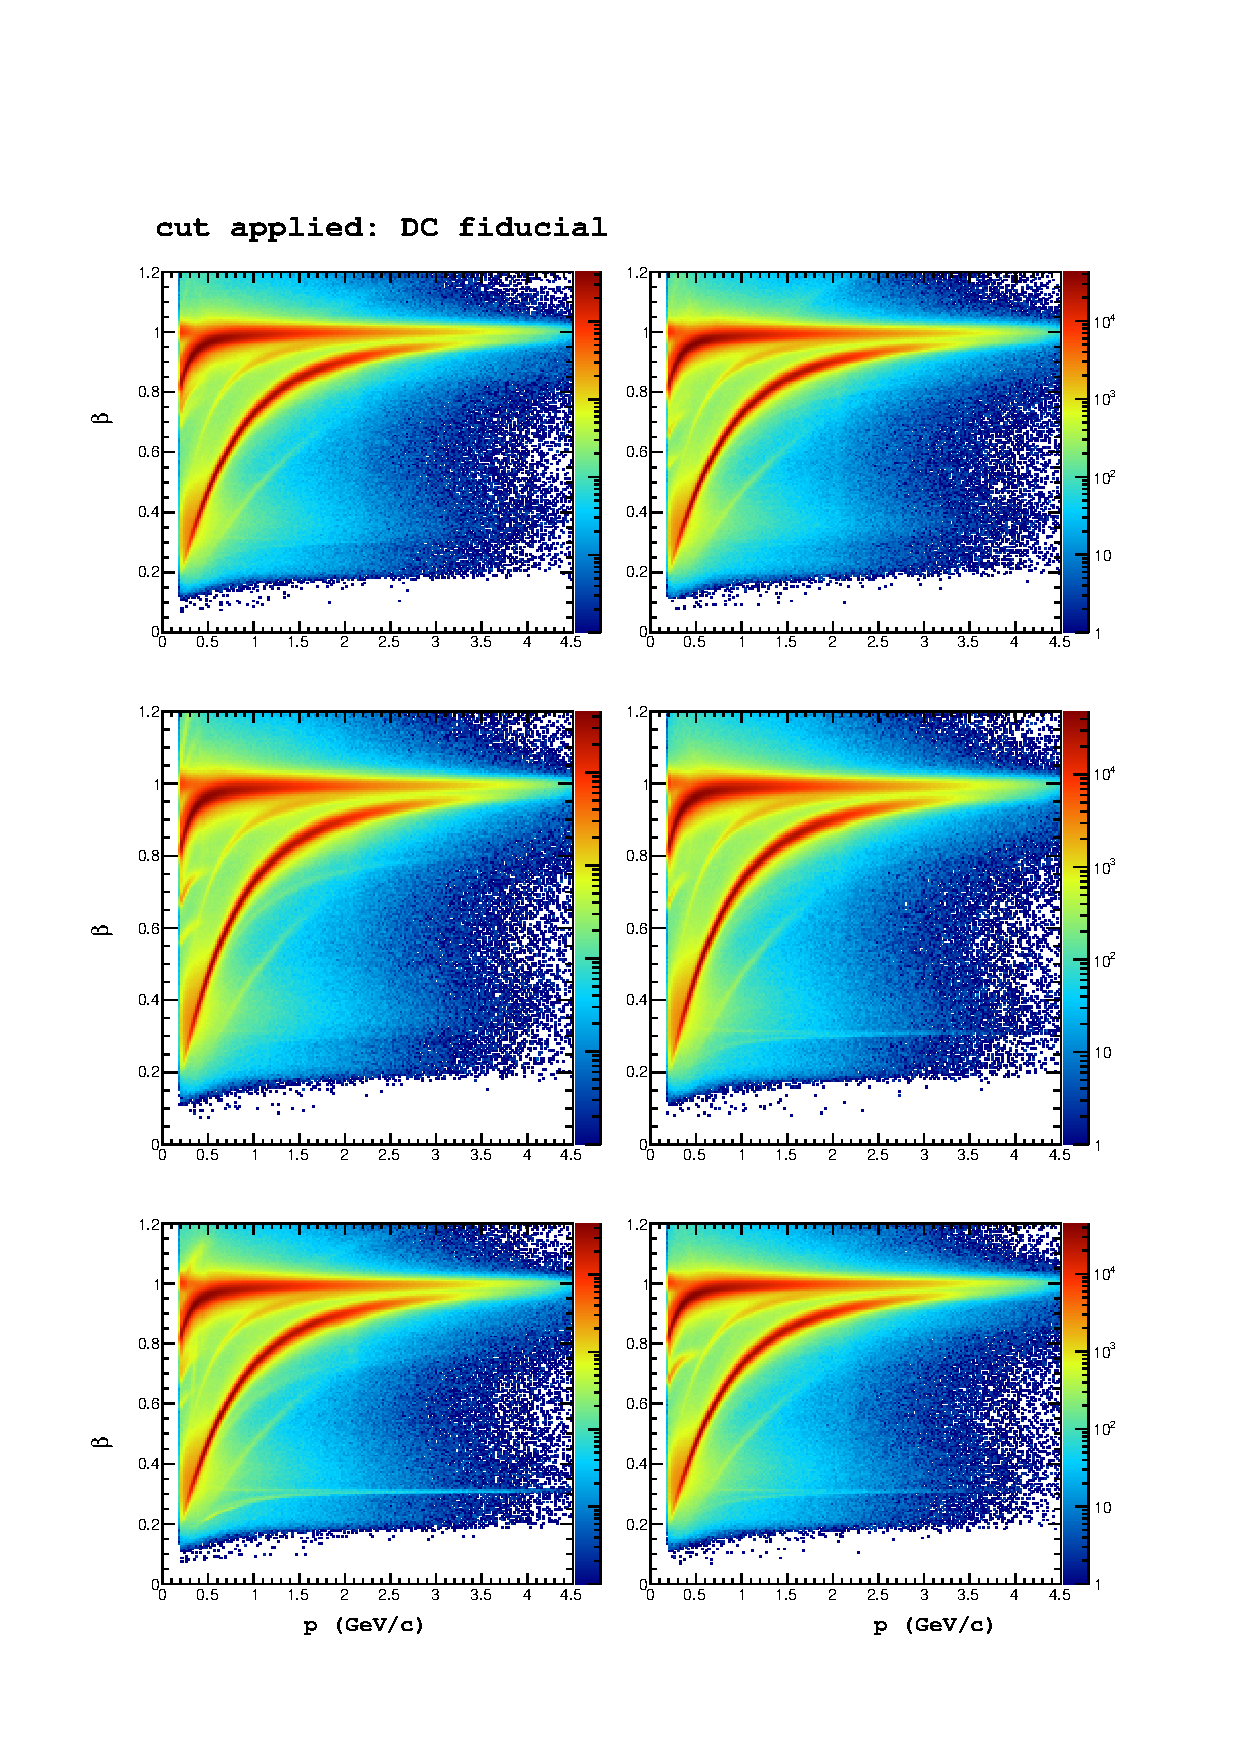
\includegraphics[width=10cm]{image/p_beta_fid.pdf}
%    \caption{Shown above: }
%  \end{center}
%\end{figure}

\subsubsection*{Likelihood maximization of $\beta(p,h)$}
In this section, positive hadrons are used as an example.  For each particle species considered, a normalized probability density function $P(x;p,h)$ is constructed for each input into the likelihood analysis.  Here, $x$ corresponds to the feature being used to categorize different particles (in our case, $x$ is the $\beta$ value measured by CLAS time-of-flight), $p$ is the particle momentum, and $h$ is the label for the hadron being hypothesized (eg: the possible values for positive hadrons are pion, kaon, proton).  In general if one uses a set of $N$ variables $x = (x_1, x_2, ..., x_N)$, the likelihood for a hypothesis $h$ is defined below.

\begin{equation}
  \mathcal{L}_h = \prod^{N}_{i=1} P_{i} (x_i; p, h)
\end{equation}

In our case, the only random variable we consider is $\beta$, and the likelihood is just the PDF.  Here, and in many cases where the choice is statistically appropriate, it is possible to use a Gaussian PDF for the variable $x_i$ (here $\beta$).  The variable $\sigma_{\beta} (p,h)$ is the standard deviation of the PDF at a given value of momentum and for a given hadronic species, similarly $\mu_{\beta}$ is the mean of the Gaussian PDF for the same value of momentum and same hadron. 

\begin{equation}
  P(\beta;p,h) = \frac{1}{\sqrt{2 \pi} \sigma_\beta(p,h) } exp \left \{ -\frac{1}{2} \bigg( \frac{\beta - \mu_\beta(p,h)}{\sigma_\beta(p,h)} \bigg)^2 \right \}
\end{equation}

The identity is assigned by choosing the particle hypothesis h which maximizes the likelihood ratio.  
 
\begin{equation}
  \frac{\mathcal{L}_h}{\mathcal{L}_{\pi}+\mathcal{L}_{K}+\mathcal{L}_{p}}
\end{equation}

Using this method, every positive track is assigned a particle identification.  However, at times the likelihood value is quite small when compared with the maximum likelihood for that species.  This is the case for positrons which are classified by this method as positive pions, because they are the closest particle for which a hypothesis has been provided.  To avoid these situations, the confidence level $\alpha$ of each track is calculated and a cut is applied on the minimum confidence.  This cut can be easily varied to see how it changes the analysis result.

\begin{equation}
  \alpha = 1 - \int_{\mu-\beta_{obs}}^{\mu+\beta_{obs}} P(\beta;p,h) d\beta
\end{equation}

This quantity represents the probability to observe a value of $\beta$ as far or farther from the mean as $\beta_{obs}$.  Confidence levels close to zero correspond to tracks which are poorly identified as the class h.  In the case that the PDF is Gaussian, the standard 1, 2, and 3 $\sigma$ cuts on $\beta$ vs. $p$ can be understood simply as confidence levels of approximately 0.32 = 1-0.68, 0.05 = 1-0.95, and 0.01 = 1-0.99.

\begin{figure}
  \begin{center}
    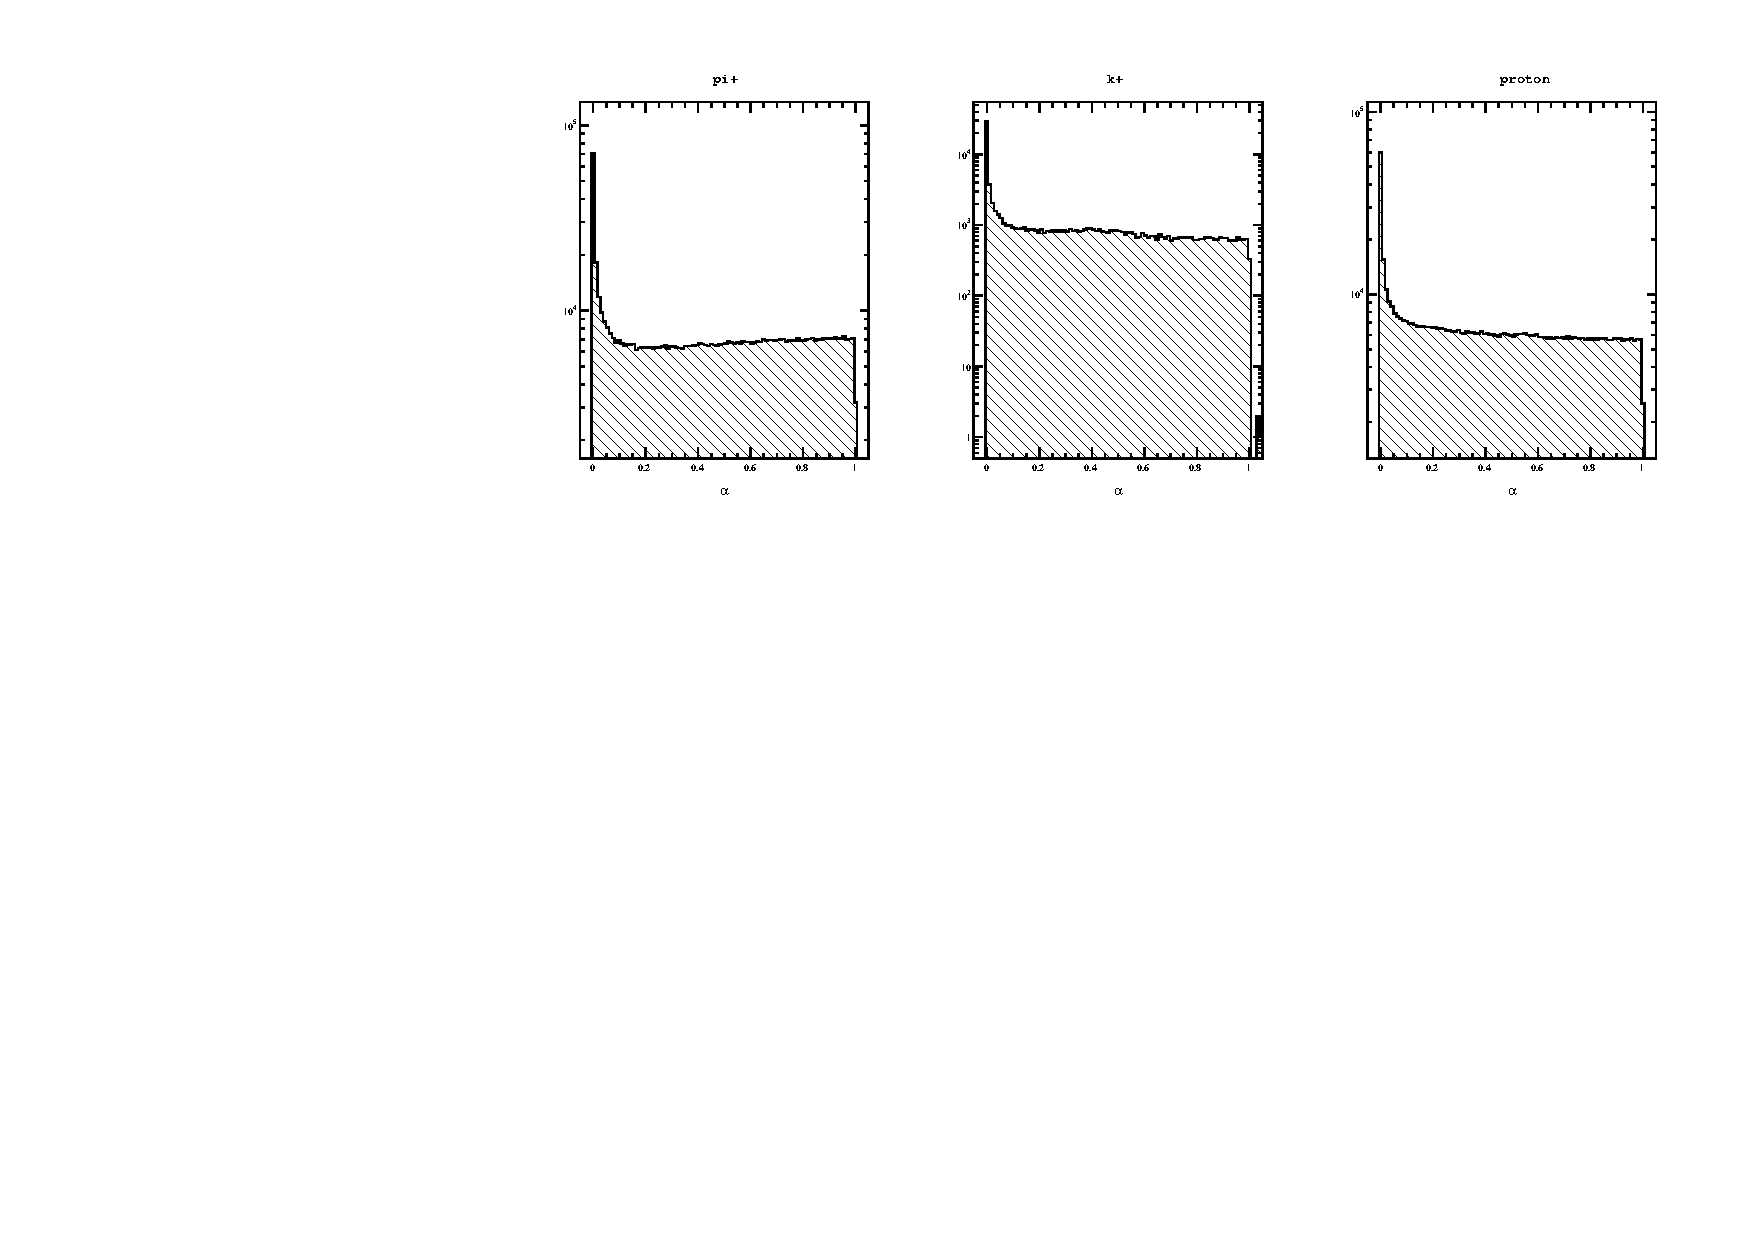
\includegraphics[width=16cm]{image/plots/hadron-id/confidence_level.pdf}
    \caption{ Shown above: The distribution of confidence level for all positive tracks after being classified by the likelihood ratio.}
  \end{center}
\end{figure}

\subsubsection*{Determination of probability density functions for likelihood method}

The most important and most difficult part of constructing the likelihood ratio identification is the determination of the mean and standard deviation of the probability density function (which depends on momentum) for the different hypotheses.  In the case where exceptionally accurate monte carlo (MC) simulations of the detector are available, one can use the truth information and track matching to construct the $\beta$ vs. $p$ 2-dimensional histograms, and fit the $\mu(p)$ and $\sigma(p)$.  In the absence of high quality MC, analysts typically fit directly the spectrum of $\beta$ vs. $p$ and extract the mean and variance.  In this work, an enhanced sample of candidates for each of the three positive particles in question is created before doing the fitting.  In this way, we hope that our fit better represents the true $\mu$ and $\sigma$ for each particle.  For fitting of pion and proton resolutions, positive tracks are assumed to be pions and the missing mass of the event is calculated.  Then, a cut is placed around the neutron mass.  In doing so, two main exclusive reactions are selected.  The first is $ep \rightarrow e\pi^+N$, and the second is $ep \rightarrow ep\pi^0$.  In this way most positrons, and positive kaons are removed from the sample prior to fitting.  The mean and variance are fit using a third order polynomial in p (MINUIT $\chi^2$ minimization is used).  For accessing the kaon distribution, the opposite condition is applied.  This is not nearly as effective as the pion case, but we believe is still an improvement over fitting the spectrum directly.    

\begin{figure}
  \begin{center}
    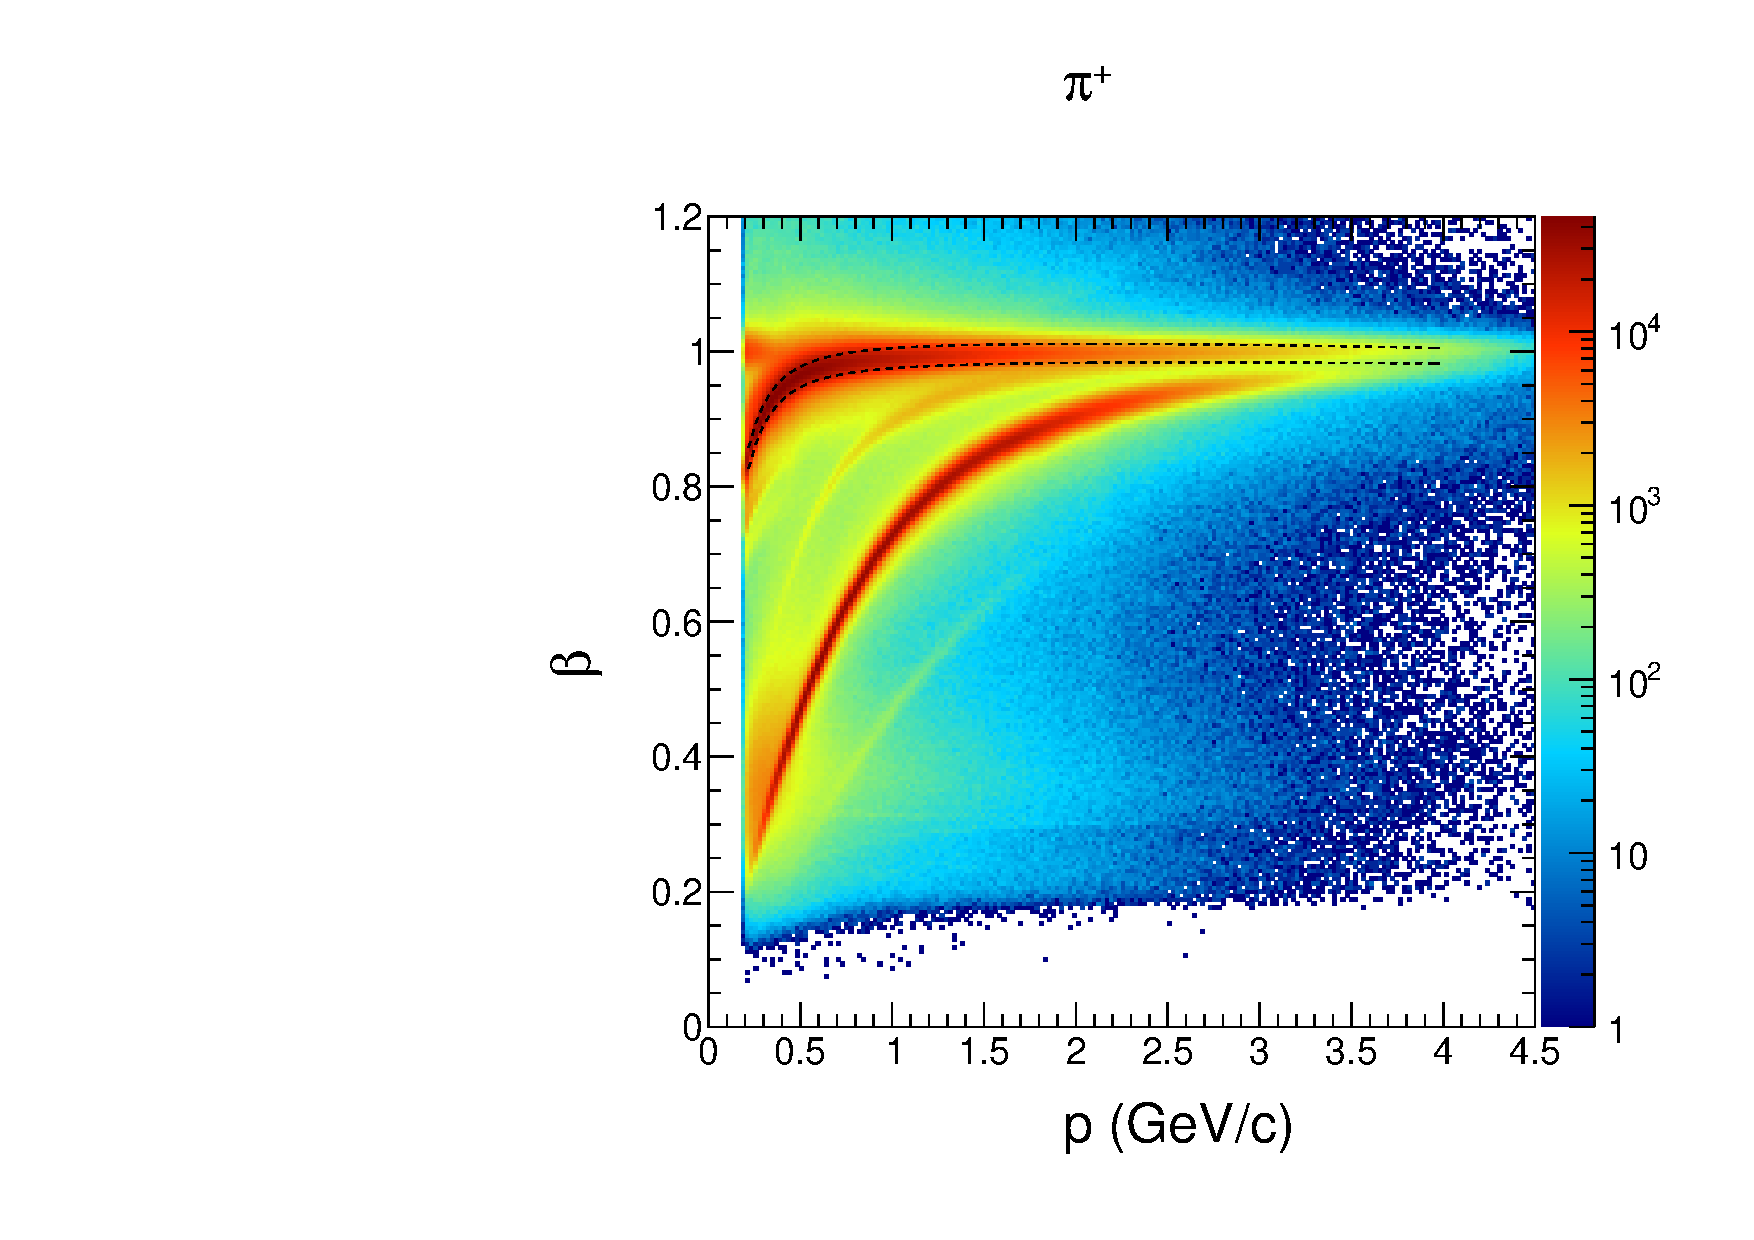
\includegraphics[width=10cm]{image/plots/hadron-id/beautiful_pbeta_pip.pdf}
    \caption{All positive tracks overlaid with our determination of $\mu(p) \pm \sigma(p)$ for $\pi^+$ (black dashed lines).}
  \end{center}
\end{figure}

\begin{figure}
  \begin{center}
    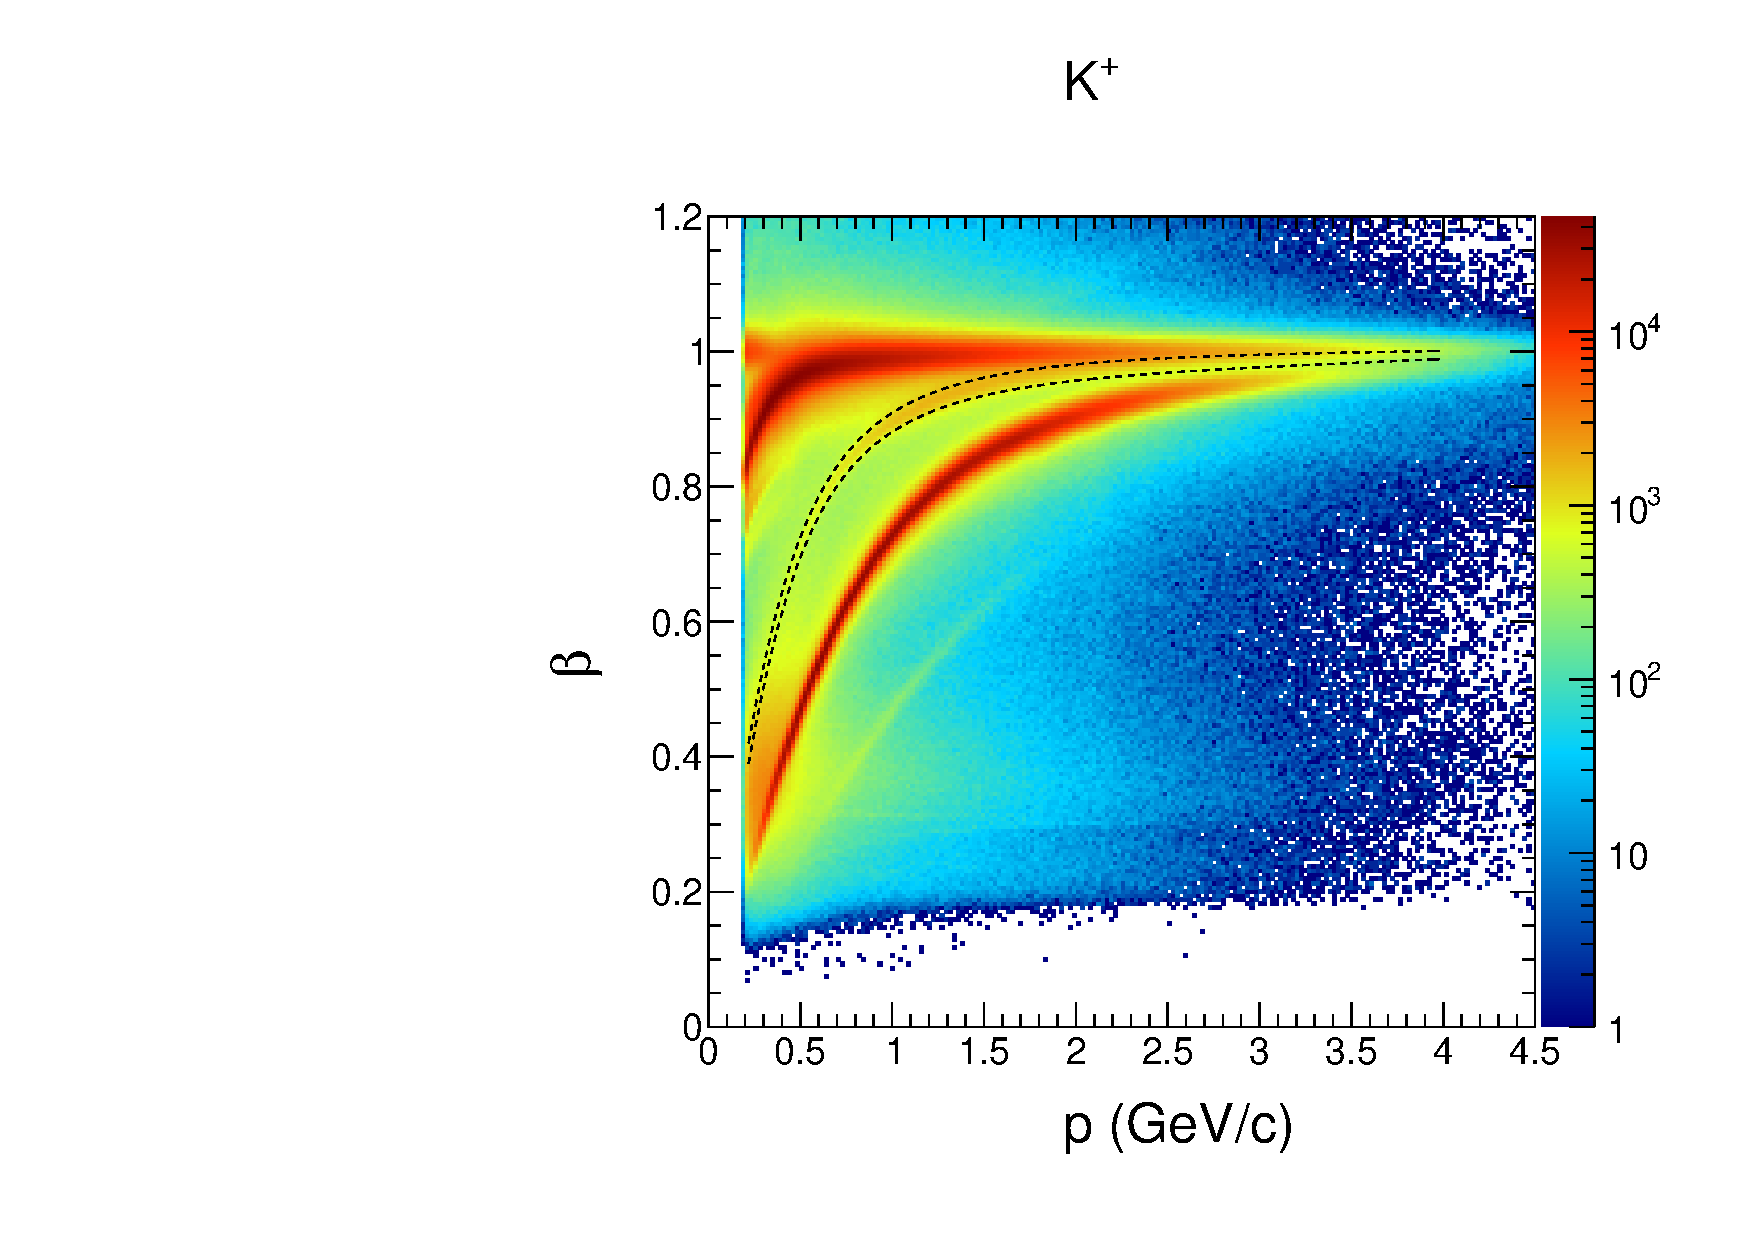
\includegraphics[width=10cm]{image/plots/hadron-id/beautiful_pbeta_kp.pdf}
    \caption{All positive tracks overlaid with our determination of $\mu(p) \pm \sigma(p)$ for $K^+$ (black dashed lines).}
  \end{center}
\end{figure}

\begin{figure}
  \begin{center}
    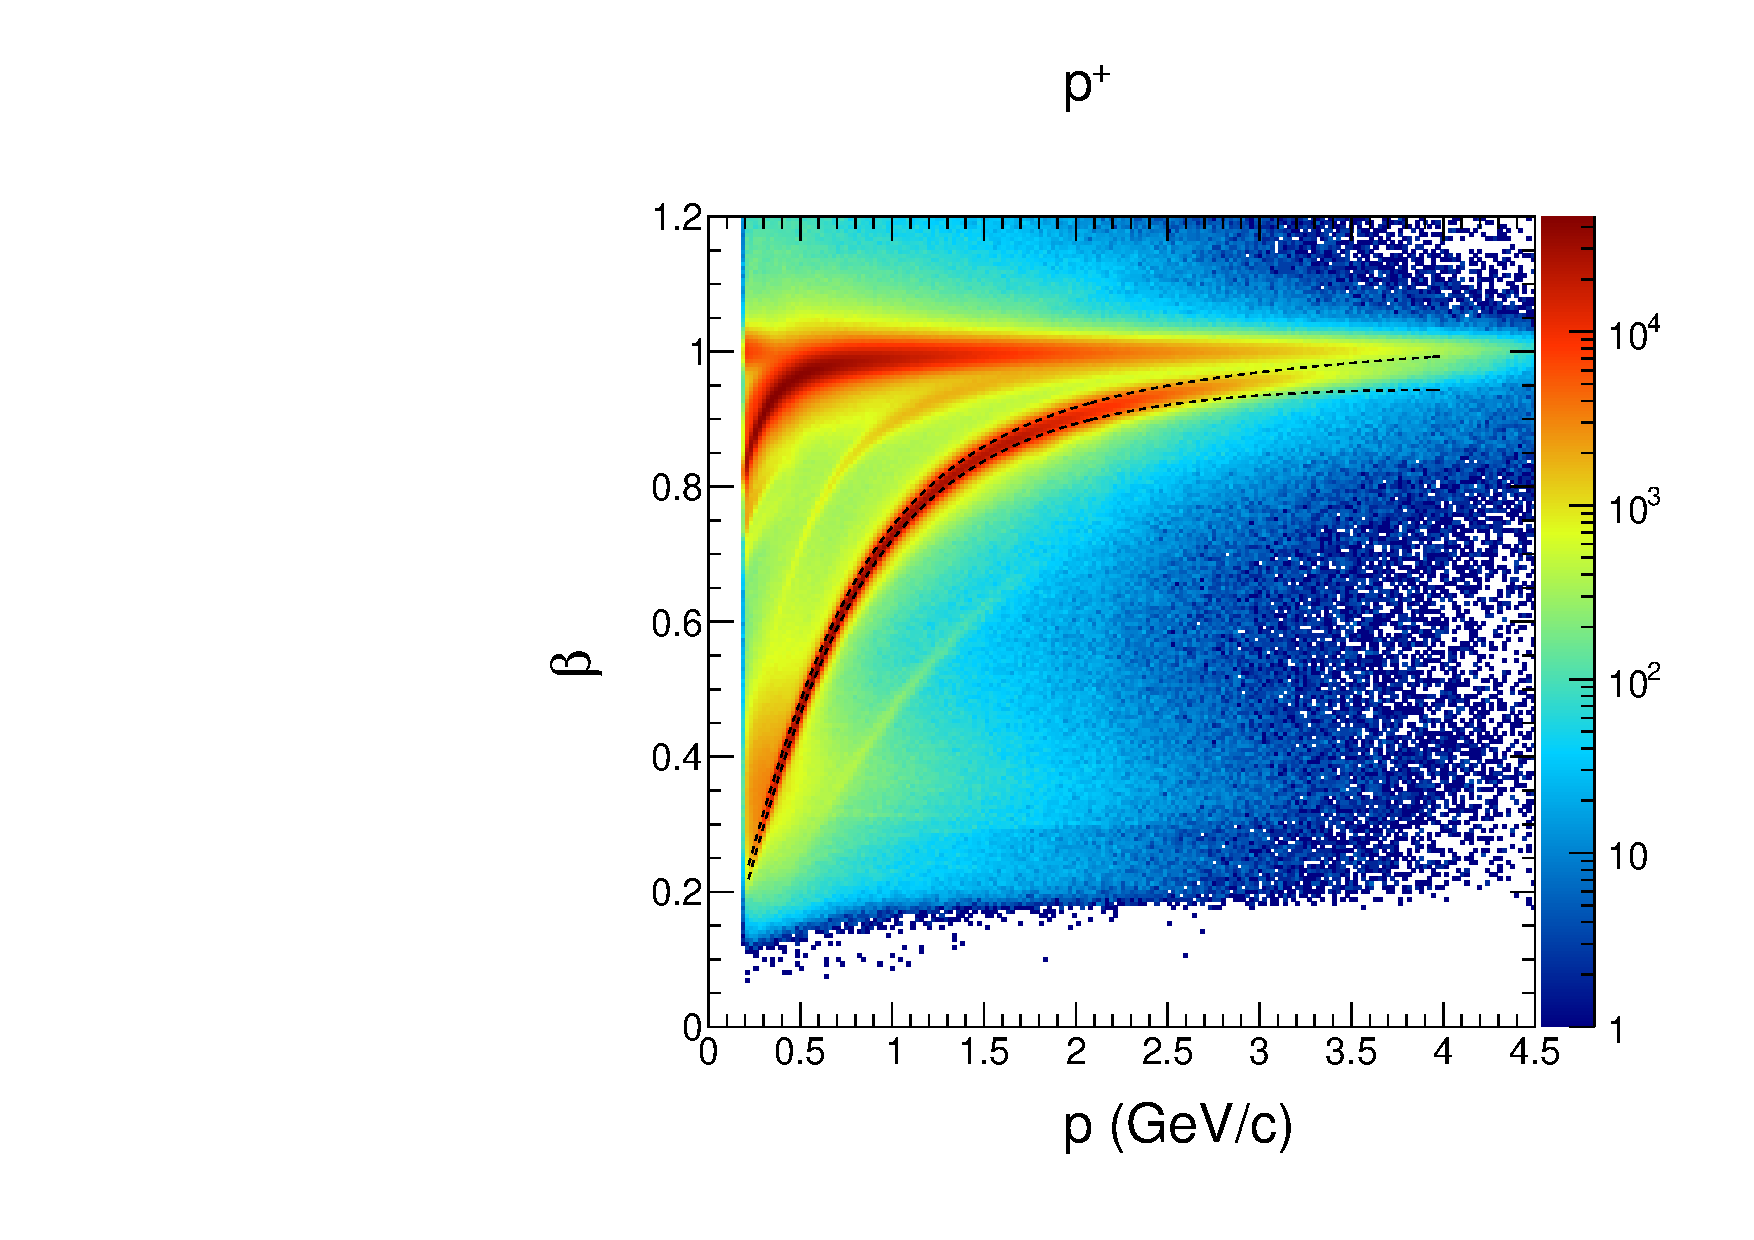
\includegraphics[width=10cm]{image/plots/hadron-id/beautiful_pbeta_prot.pdf}
    \caption{All positive tracks overlaid with our determination of $\mu(p) \pm \sigma(p)$ for $p^+$ (black dashed lines).}
  \end{center}
\end{figure}

The parametrization used for the mean $\mu_ (p,h)$ and resolutions $\sigma (p,h)$ are shown below.

\begin{eqnarray}  
  \mu (p,h) = \mu_{theory} + \Delta \mu       \\
  \mu_{theory} = \frac{1}{\sqrt{1+(m_h/p)^2}} \\
  \Delta \mu = \mu_0 + \mu_1 p + \mu_2 p^2    \\
  \sigma (p,h) = \sigma_0 + \sigma_1 p + \sigma_2 p^2
\end{eqnarray}

The values are displayed in the table below. 

\begin{landscape}
  \begin{table}
%  \centering
  \begin{tabular}{c|c|c|c|c|c|c|c}
    Hadron & Parameter & Sector 1 & Sector 2 & Sector 3 & Sector 4 & Sector 5 & Sector 6 \\
    \hline 
      $K^+$ & $\mu_2$ & 0.00111554 & -8.97687e-05 &        4.78796e-05 &        0.000376425 &        -0.00204856 &        0.000652209 \\
       $K^+$ & $\mu_1$ & -0.00468038 & 6.19414e-05 &        -0.00081741 &       -0.00107931 &         0.00629181 &        -0.00264143 \\
       $K^+$ & $\mu_0$ & 0.00361012 &         0.00134921 &         0.00299674 &         0.00220194 &        0.000117821 &         0.00162582 \\
    $K^+$ & $\sigma_2$ & -0.000331838 &        -0.00105807 &       -0.000712404 &       -0.000573934 &       -0.000259289 &        0.000508389 \\
    $K^+$ & $\sigma_1$ & -0.00105857 &         0.00236686 &        0.000509169 &        0.000163467 &        -0.00233617 &        -0.00461598 \\
    $K^+$ & $\sigma_0$ & 0.0154964 &           0.0117702 &          0.0140748 &          0.0143761 &          0.0184055 &         0.0180945 \\
      $\pi^+$ & $\mu_2$ & -0.000962041 &       -0.000300602 &       -0.000306326 &        -3.2245e-05 &        -0.00226511 &       -0.000330818 \\
      $\pi^+$ & $\mu_1$ & 0.00296349 &          0.0016512 &          0.0021962 &         0.00176045 &         0.00750862 &         0.00126443 \\
      $\pi^+$ & $\mu_0$ & -0.00225794 &        -0.00047045 &        0.000370406 &        0.000435526 &       -0.000449409 &        -0.00131045 \\
   $\pi^+$ & $\sigma_2$ & -0.000127659 &        0.000691895 &       -0.000289961 &        0.000315041 &       -0.000936521 &       -0.000131269 \\
   $\pi^+$ & $\sigma_1$ & -0.000489092 &         -0.0033948 &         0.00196853 &       -0.00197841 &         0.00212778 &       -0.000339411 \\
   $\pi^+$ & $\sigma_0$ & 0.0155195 &           0.0167998 &          0.0124066 &          0.0157476 &          0.0145571 &         0.0141728 \\
     $p^+$ & $\mu_2$ & -0.00039358 &       -0.000701003 &       -0.000347651 &          0.0004854 &        -0.00121666  &       0.000563786 \\
     $p^+$ & $\mu_1$ & -0.000295423 &         0.00170899 &        0.000794901 &       -0.000744446 &         0.00376887 &        -0.00353545 \\
     $p^+$ & $\mu_0$ & 0.00227353 &         0.00231676 &         0.00364672 &         0.00276859 &         0.00128827 &          0.00439605 \\
  $p^+$ & $\sigma_2$ & 0.001429 &         0.00144256 &         0.00124456 &         0.00190709 &         0.00141039 &          0.0011516 \\
  $p^+$ & $\sigma_1$ & -0.0021472 &        -0.00262226 &        -0.00196308 &        -0.00385218 &        -0.00186708 &        -0.00186749 \\
  $p^+$ & $\sigma_0$ & 0.0107541 &          0.0109091 &          0.0104381 &          0.0115449 &          0.0109969 &          0.0107759 
  \end{tabular}
  \caption{Values used to calculate the mean and resolution for hadron likelihood based identification.}
  \label{table-hadron-pdfs}
  \end{table}
\end{landscape}

\subsubsection*{Validation of Kaon Identification}
A Monte Carlo simulation was used to study particle identification of positive hadrons as a function of the hadronic momentum.  As a result of this study the minimum confidence level ($\alpha = 0.55$) and maximum momentum ($p_{max} = 2.0 \; GeV/c$) for $K^+$ were determined. \\

To study this SIDIS events were generated using \texttt{clasdis}.  Our simulation includes $\pi^+$, $K^+$ and protons (here denoted $P^+$) over a range of kinematics consistent with the E1-F beam energy of $E_{beam} = 5.498 \; GeV$.  After passing these events through the CLAS detector simulation \texttt{GSIM}, reconstruction was used to fit tracks.  The truth information for generated kinematics was stored in the output files, and we correlated reconstructed particles to their generated counter-part by requiring that magnitude of the three momentum difference was small ($\delta P < 0.05$).  

\begin{equation}
	\delta P = \frac{|\vec{P_{gen}} - \vec{P_{rec}}|}{|\vec{P_{gen}}|}
\end{equation}   

In this simple equation $P_{rec}$ and $P_{gen}$ are the reconstructed and generated three momentum of the track being matched.  After this matching procedure has been applied, we calculate two simple metrics, the \textit{purity} and the \textit{efficiency}.  The purity refers to the fraction of tracks that are classified as kaons that are truly kaons.  More formally it is written, 

\begin{equation}
		P = \frac{tp}{tp + fp} = \frac{N_{K^+}}{N_{K^+} + N_{\pi^+} + N_{P^+}}
\end{equation}     

where $tp$ and $fp$ are true positives and false positives respectively, and the variables $N$ refer to the true number of tracks with that label in the sample.  The efficiency is simply the fraction of all true kaons which are identified as kaons, and can be written as shown below.   

\begin{equation}
	\epsilon = \frac{tp}{tp + fn} = \frac{N_{K+^}^{identified}}{N_{K^+}^{total}}
\end{equation}

As a simple illustrative example, consider the case when all hadrons are called kaons, in this case the efficiency is 1, but the purity will be at its minimum (related to the fraction of total particles that are kaons).  As the purity of the sample is increased, the efficiency drops.  For this study the efficiency drives our statistical errors, but the purity is the more important metric.  As the cut boundaries are restricted by raising the minimum confidence level of hadrons identified as kaons, the purity goes up and the efficiency goes down \ref{fig:kaon_efficiency_purity}.

\begin{figure}
	\centering
	\label{fig:beta_p_simulation}
	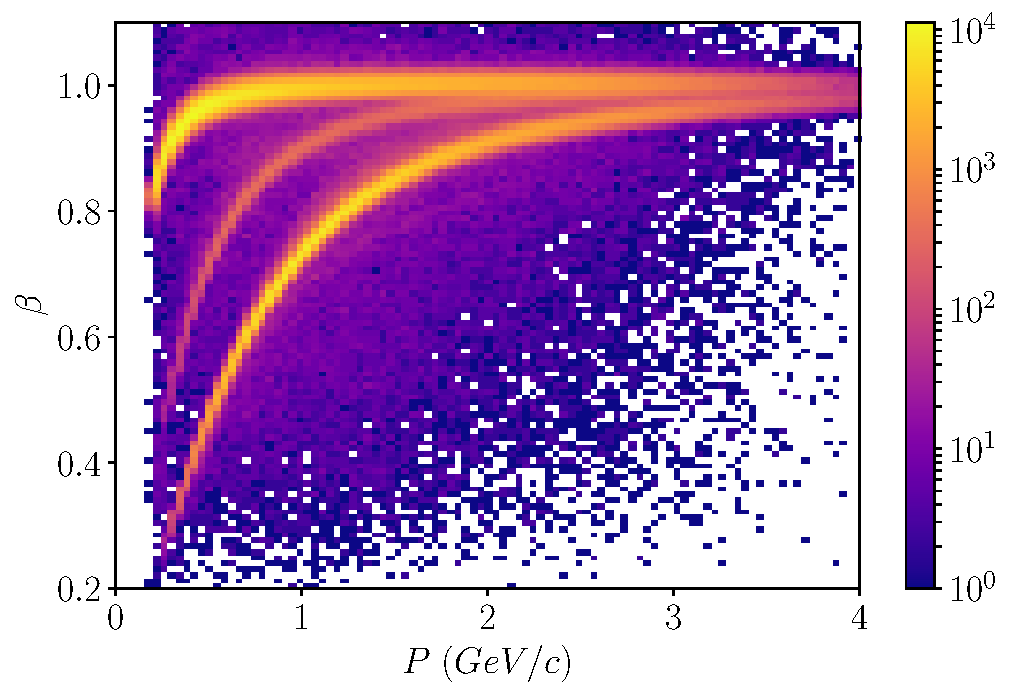
\includegraphics[width=15cm]{image/plots/hadron-id/beta_p_simulation.pdf}
	\caption{Positive hadrons from the Monte Carlo simulation produce a $\beta$  vs. p simulation that is very similar to data.}
\end{figure}

\begin{figure}
	\centering
	\label{fig:kaon_efficiency_purity}
	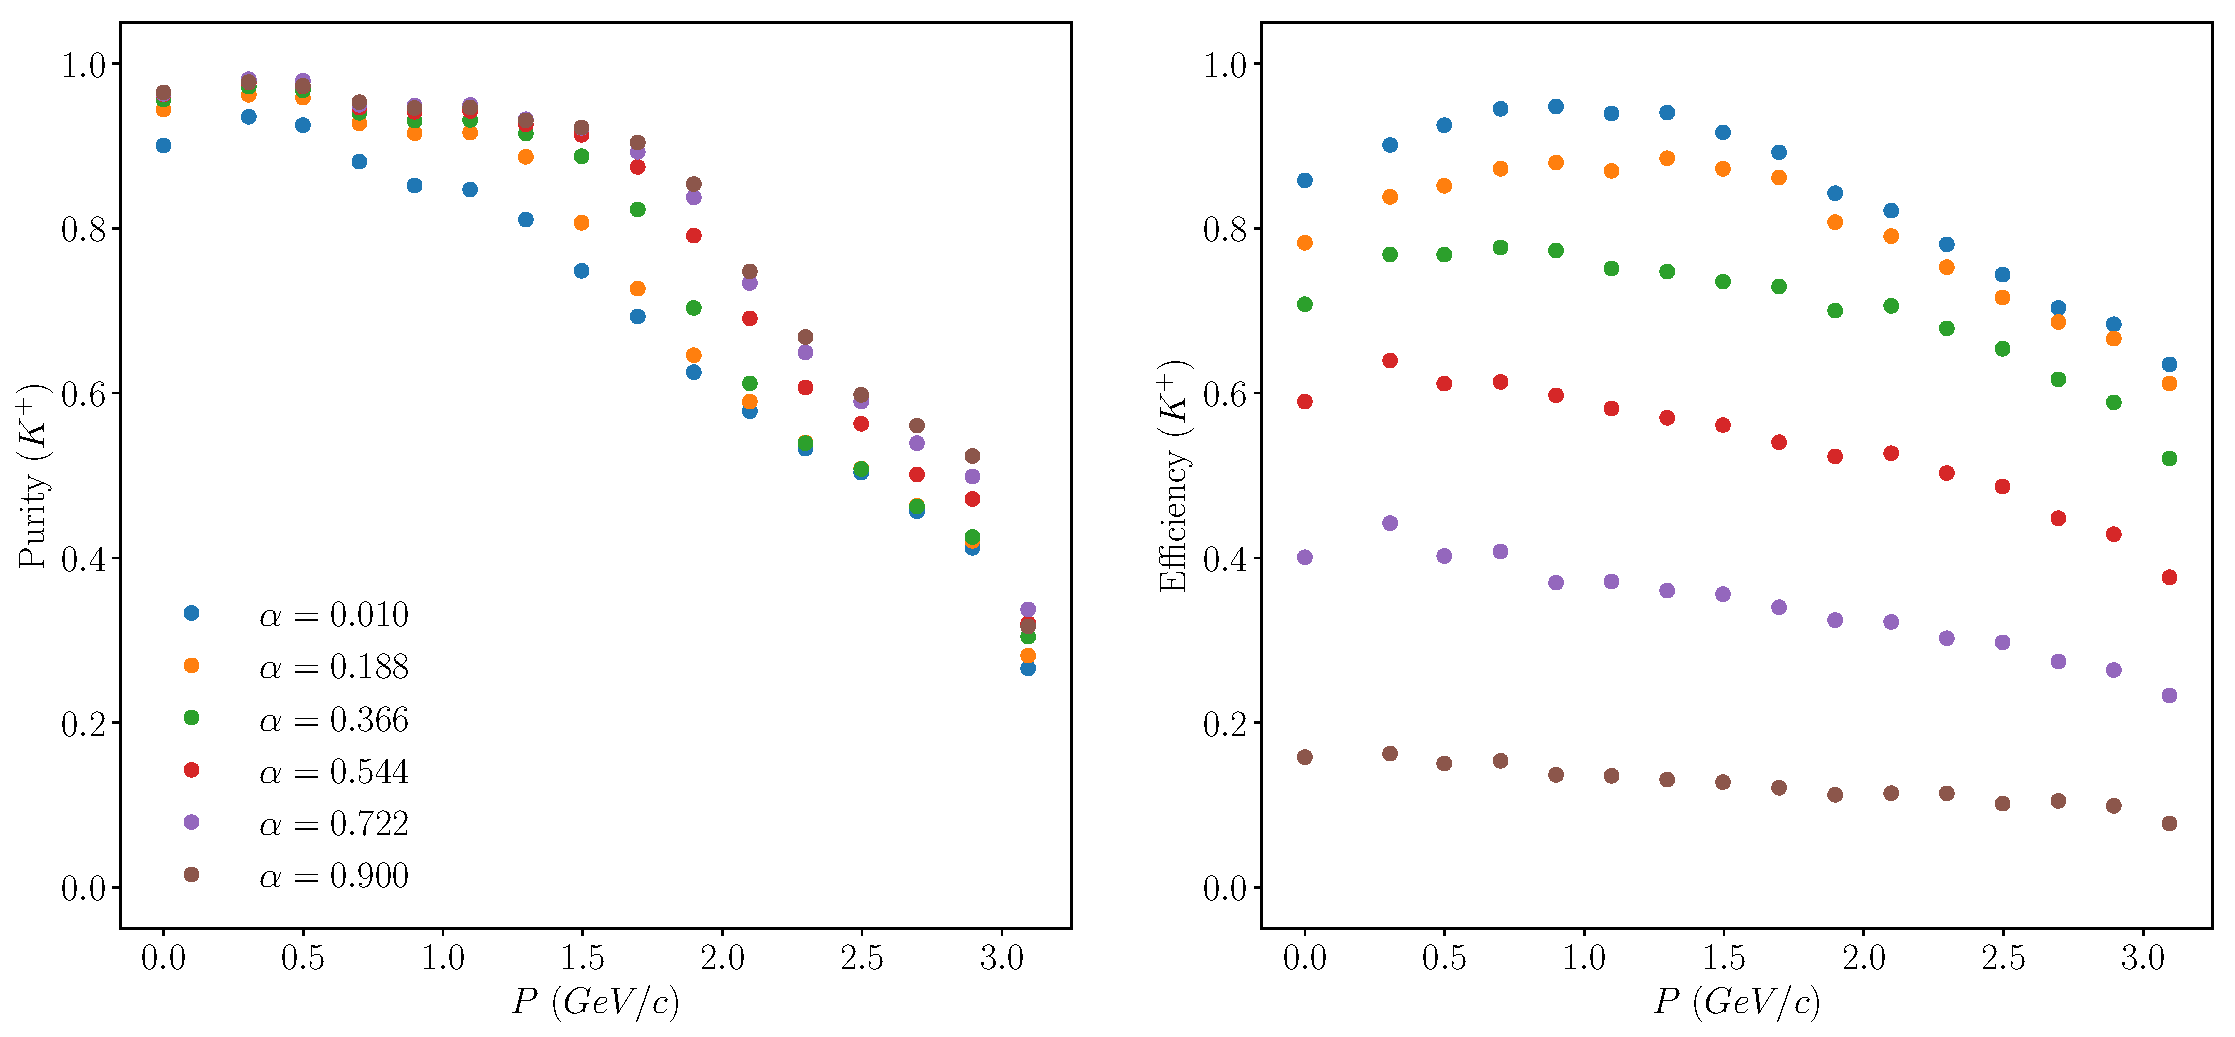
\includegraphics[width=15cm]{image/plots/hadron-id/kaon_efficiency_purity.pdf}
	\caption{The efficiency and purity of our kaon sample are studied by using a Monte Carlo simulation.  Here, the results are studied as a function of the confidence level, and of the track momentum.}
\end{figure}

Based on this study, a maximum momentum of 2.0 GeV and a minimum confidence $\alpha_{min}$ of 0.55 is required for all kaons in our analysis, which provides a purity of 80\% or more (depending on the kinematics).  The magnitude of the $\pi^+$ asymmetry is known in these kinematics to be on the order of 0.02, if the sample is comprised of 20\% pions (which is the worse case in our measurement) then the contribution to the total asymmetry is equivalent to a $K^+$ asymmetry of 0.005, which is much smaller than our errors.  This level of contamination is therefore very tolerable, and should have no significant impact on our analysis.  
